\documentclass[<options>]{article}
\RequirePackage{amsfonts,amssymb,amsbsy,amsmath}
\usepackage{epsfig,longtable}
\usepackage{listings}
\usepackage{textcomp}
%\usepackage[pdftex]{graphicx}
\textheight     9.0in \textwidth      6.0in \oddsidemargin  0.0in
\evensidemargin 0.0in \topmargin      -.2in
\parskip        6pt

\DeclareMathOperator{\diag}{diag}

\def\bb{{\beta}}
\def\b{\mbox{\boldmath$\beta$}}
\def\x{\mbox{\boldmath$\xi$}}
\def\no{\noindent}
\def\DD{{\Delta}}
\def \Ac {{\cal A}}



\newtheorem{theo}{Theorem}[section]
\newtheorem{cor}{Corollario}[section]
\newtheorem{lem}{Lemma}[section]
\newtheorem{defn}{Definition}[section]
\newtheorem{ex}{\small \bf Esercizio}[section]
\newtheorem{exa}{\sc \bf Example}[section]
\newtheorem{rem}{\sc Remark}[section]


\def\proof{{\bf Proof.}\quad}
\def \x {{\bf x}}
\def \a {{\bf a}}
\def \b {{\bf b}}
\def \c {{\bf c}}
\def \zero {{\bf 0}}
\def \y {{\bf y}}
\def \b {{\bf b}}
\def \f {{\bf f}}
\def \e {{\bf e}}
\def \w {{\bf w}}
\def \u {{\bf u}}
\def \v {{\bf v}}
\def \t {{\bf t}}
\def \z {{\bf z}}
\def \g {{\bf g}}

\def \xs {{\bar {x}}}
\def \ys {{\bar {y}}}
\def \gs {{\bar {\gamma}}}
\def \ml {{|\lambda|}}
\def \CC {{\mathbb{C}}}
\def \RR {{\mathbb{R}}}
\def \ZZ {{\mathbb{Z}}}
\def \NN {{\mathbb{N}}}
\def \barD {{  \overline  \Delta}}



\def \doty {\dot {\bf {y} }}
\def \ddoty {\ddot {\bf {y} }}
\def \dotv {\dot {\bf {v} }}
\def \eps {\varepsilon}
\def \lt {\tilde{\lambda}}
\newcommand{\balpha}{\mbox{\boldmath $\alpha$}}
\newcommand{\bbeta}{\mbox{\boldmath $\beta$}}
\newcommand{\bdelta}{\mbox{\boldmath $\delta$}}
\newcommand{\brho}{\mbox{\boldmath $\rho$}}
\newcommand{\btau}{\mbox{\boldmath $\tau$}}
\newcommand{\bxi}{\mbox{\boldmath $\xi$}}
\newcommand{\cbxi}{\mbox{\boldmath $\hat \xi$}}

\def \no {\noindent}



\def \pmatrix{ \left( \begin{array} }
\def \endpmatrix{ \end{array} \right) }
\hyphenation{me-thod} \hyphenation{me-thods} \hyphenation{exact}
\hyphenation{ar-bi-tra-ri-ly} \hyphenation{dia-go-nal-ly}

\lstset{language=MATLAB}
\lstset{commentstyle=\textit,upquote=false}
\lstset{basicstyle=\small}
\lstloadlanguages{MATLAB}

\begin{document}


\vspace*{1cm}

\begin{center}
{\Huge BVPTWP Package:\\ solving test problems}\\[5mm]
{\Large J. R. CASH$^{\ast}$, D. HOLLEVOET$^{\star}$, F. MAZZIA$^{\dag}$,  A. M. NAGY$^{\ddagger}$}\\
[5mm]
{\Large $^{\ast}$\small Department of Mathematics,
Imperial College, South Kensington, London SW7, England.}\\ e-mail: \texttt{j.cash@imperial.ac.uk}\\[5mm]
{\Large $^{\star}$\small Vakgroep Toegepaste Wiskunde en Informatica, Universiteit Gent, Krijgslaan 281 S9, 9000 Gent.}\\
e-mail:
\texttt{davy.hollevoet@ugent.be}\\[5mm]
{\Large $^{\dag}$\small Dipartimento di Matematica, Universit\`a di Bari, Via Orabona 4, 70125 Bari (Italy).}\\
e-mail:
\texttt{mazzia@dm.uniba.it}\\[5mm]
{\Large $^{\ddagger}$\small Dipartimento di Matematica, Universit\`a di Bari, Via Orabona 4, 70125 Bari (Italy)\\ Department of Mathematics, Benha University, 13518 Benha (Egypt). } \\
e-mail: \texttt{abdelhameed\_nagy@yahoo.com}\\
\end{center}


\newpage
\section*{Contents}
\begin{tabular*}{\textwidth}{@{}lcrcr@{}}
\multicolumn{5}{@{}c@{}}{\rule{\textwidth}{0mm}}\\
\phantom{I}1.\; Introduction                       &&&& {\sl \pageref{intro}} \\[2mm]
\phantom{I}2.\; Format of the problem codes     &&&& {\sl \pageref{Format}} \\[2mm]
\phantom{II}2.1.\; The function prob                     &&&& {\sl \pageref{prob}} \\[2mm]
\phantom{II}2.2.\; The function fun    &&&& {\sl \pageref{fun}} \\[2mm]
\phantom{II}2.3.\; The function bcfun     &&&& {\sl \pageref{bcfun}} \\[2mm]
\phantom{II}2.4.\; The function dfun     &&&& {\sl \pageref{dfun}} \\[2mm]
\phantom{II}2.5.\; The function dbcfun     &&&& {\sl \pageref{dbcfun}} \\[2mm]
\phantom{II}2.6.\; The function settolerances     &&&& {\sl \pageref{settol}} \\[2mm]
\phantom{II}2.7.\; The function setoutput    &&&& {\sl \pageref{setout}} \\[2mm]
\phantom{II}2.8.\; The function esolu     &&&& {\sl \pageref{esolu}} \\[2mm]
\phantom{I}3.\; How to solve test problems with driver function    &&&& {\sl \pageref{driver}} \\[2mm]
\phantom{I}4.\; Linear Problems    &&&& {\sl \pageref{Linear}} \\[2mm]
\phantom{I}5.\; Nonlinear Problems    &&&& {\sl \pageref{Nonlinear}} \\[2mm]
%\multicolumn{5}{c}{\pmb{\em Test problems collected so far:}}\\[3mm]
\end{tabular*}
\section{Introduction}\label{intro}
\texttt{bvptwp} is a MATLAB program that calculates approximate solutions
two point Boundary Value Problems. These problems may or may not be singularly perturbed.
The BVPs are of the general form:
\begin{equation}\label{bvp1}
y'=f(x,y), \quad  a \leq  x \leq b
\end{equation}
\begin{equation}\label{bvp2}
g(y(a),y(b)) = 0,
\end{equation}
where $ g = ( g_{1}, g_{2},\cdot\cdot\cdot,g_{n})^{T}$ is a vector functions.
The functions $f$ and $g_{i}$ are assumed to be differentiable.
The problem must be posed as a first-order system. This requirement is not unduly restrictive,
however, since standard techniques can be used to convert an $n$th-order equation to a system
of $n$ first-order equations. For example, the second-order   singularly
perturbed  problem
\begin{equation}
 \lambda y''=f(x,y,y'),\quad 0 < x < 1, \quad y(0) = \alpha, \quad y(1) = \beta,
\end{equation}
where $0 <\lambda \ll 1,\, x \in \mathbb{R},\,$
can be converted to the following first-order system:
\begin{equation*}
\begin{array}{l}
u' = z, \\
z' = \dfrac{1}{\lambda}f(x,u,z), \\
 u(0) = \alpha,u(1) = \beta.\\
\end{array}
\end{equation*}

\section{Format of the problem codes}\label{Format}
The eight functions that define the problem are called \texttt{prob},
\texttt{fun}, \texttt{bcfun}, \texttt{dfun}, \texttt{dbcfun},  \texttt{settolerances},
\texttt{setoutput} and \texttt{esolu}. The following subsections describe the
format of these subroutines in full detail.
\subsection{The function prob}\label{prob}
This routine gives some general information about the test
problem.
\begin{verbatim}
function [problm,type,m,Linear,numjac,numbcjac,Vectorized,JVectorized,solinit]=prob()
\end{verbatim}
Meaning of the arguments:
\begin{list}
{}{%
  \renewcommand\makelabel[1]{\texttt{#1}\hfill}
}
\item[problem]\ \\
This character string contains the name of the problem, e.g.\ \texttt{bvpT1}, and
corresponds to the name of the MATLAB source file.
\item[type]\ \\
This character string takes the value \texttt{ODEBVP}.
%\item[t]\ \\
%An array containing time points.
\item[m]\ \\
The dimension of the problem, which is the number of equations to be solved.
%\item[nlbc]\ \\
%The number of boundary conditions at the left, the number of the right being equal to  \texttt m-nlbc.
\item[Linear]\ \\
Display if the problem is linear or nonlinear. Using 'on' the problem is treated as linear and 'off' for nonlinear.
\item[numjac]\ \\
Specify if the problem can be solved by using the analytic Jacobian (numjac =0)  or by computing it numerically (numjac =1).
\item[numbcjac]\ \\
Specify if the problem can be solved by using the analytic partial derivative of the boundary condition (numbcjac = 0) or by computing it
numerically (numbcjac = 1).
\item[Vectorized]\ \\
The solver can use the option  \texttt Vectorized  'on' or 'off' to reduce the number of function evaluations required.
By default,  \texttt Vectorized  is 'on'.
\item[JVectorized]\ \\
The solver can use the option  \texttt JVectorized  'on' or 'off' to reduce the number of function evaluations required.
By default,  \texttt JVectorized  is 'on'.
\item[solinit]\ \\
A guess for the initial mesh and the solution.
\end{list}
\subsection{The function fun}\label{fun}
This subroutine evaluates the function $f.$
\begin{verbatim}
function F = fun(X,Z,ExtraArgs)
\end{verbatim}
Meaning of the arguments:
\begin{list}
{}{%
  \renewcommand\makelabel[1]{\texttt{#1}\hfill}
}
\item[X]\ \\
The time point where the function is evaluated.
\item[Z]\ \\
The value of $y$ at which the function is evaluated.
\item[ExtraArgs]\ \\
Argument that declares the optional argument in the main program.
\item[F]\ \\
The resulting function value.
\end{list}
\subsection{The function bcfun}\label{bcfun}
This function evaluates the boundary condition.
\begin{verbatim}
function  bc = bcfun(ya,yb,ExtraArgs)
\end{verbatim}
Meaning of the arguments:
\begin{list}
{}{%
  \renewcommand\makelabel[1]{\texttt{#1}\hfill}
}
\item[ya]\ \\
Contains the left boundary condition $y(t_{0}).$
\item[yb]\ \\
Contains the right boundary condition $y(t_{n}).$
\item[ExtraArgs]\ \\
The same argument defined in the previous function.
\item[bc]\ \\
Contains the boundary value.
\end{list}
\subsection{The function dfun}\label{dfun}
This function evaluates the analytic Jacobian of The ODE function.
\begin{verbatim}
function Df = dfun(X,Z,ExtraArgs)
\end{verbatim}
Meaning of the arguments:
\begin{list}
{}{%
  \renewcommand\makelabel[1]{\texttt{#1}\hfill}
}
\item[X,Z]\ \\
The same arguments used in the function \texttt{fun}.

\item[Df]\ \\
The Jacobian value.
\end{list}
\subsection{The function dbcfun}\label{dbcfun}
This function evaluates the partial derivatives of the boundary condition.
\begin{verbatim}
function [C0,C1] = dbcfun(ya,yb,ExtraArgs)
\end{verbatim}
Meaning of the arguments:
\begin{list}
{}{%
  \renewcommand\makelabel[1]{\texttt{#1}\hfill}
}
\item[ya,yb]\ \\
The same arguments used in the function \texttt{bcfun}.
\item[ExtraArgs]\ \\
The same argument defined in the previous function.
\item[C0,C1]\ \\
Contains the partial derivatives of the boundary condition.
\end{list}
\subsection{The function settolerances}\label{settol}
This function defines the input tolerances rtol.
\begin{verbatim}
function  tolvec = settolerances(tol)
\end{verbatim}
Meaning of the arguments:
\begin{list}
{}{%
  \renewcommand\makelabel[1]{\texttt{#1}\hfill}
}
\item[tol]\ \\
Relative tolerance.
\item[tolvec]\ \\
A  vector of  tolerances that will be used in the code.
\end{list}
\subsection{The function setoutput}\label{setout}
This function contains information about the required output.
\begin{verbatim}
function [solref,printsolout,nindsol,indsol] = setoutput(plotsol)
\end{verbatim}
Meaning of the arguments:
\begin{list}
{}{%
  \renewcommand\makelabel[1]{\texttt{#1}\hfill}
}
\item[plotsol]\ \\
Index of component to be plotted (optional).
\item[solref]\ \\
Contains information about the reference solution.\\
- \texttt{solref = 1}, means that the reference solution is available.\\
- \texttt{solref = 0}, means that the reference solution is not available.
\item[printsolout]\ \\
Contains information about the required output.
\item[nindsol]\ \\
If \texttt{printsolout =1}, \texttt nindsol  contains the number of components to
be printed.
\item[indsol]\ \\
If \texttt{printsolout =1}, \texttt{indsol(1:nindsol)}  contains the index of
the \texttt nindsol  components to be printed.
\end{list}
\subsection{The function esolu}\label{esolu}
This function evaluates the exact solution of the problem if it  exists.
\begin{verbatim}
function Exact = esolu(X,ExtraArgs)
\end{verbatim}
Meaning of the arguments:
\begin{list}
{}{%
  \renewcommand\makelabel[1]{\texttt{#1}\hfill}
}
\item[Exact]\ \\
Contains the exact solution.
\item[X, ExtraArgs]\ \\
The same argument as in function \texttt{fun}.
\end{list}


%\subsection{Solver syntax}
\section{How to solve test problems with driver function}\label{driver}
From the Matlab command line the driver function can be run by calling
\begin{verbatim}
>> [sol,time] = bvpMtest(problem,solver,tol,plotsol,opts,varargin);
\end{verbatim}
The  directory  ``problems''  should  be added to the MATLAB path before
calling \texttt{bvpMtest}.

The input arguments are:
\begin{list}
{}{%
  \renewcommand\makelabel[1]{\texttt{#1}\hfill}
}
\item[problem]\ \\
The function handle of the problem.
\item[solver]\ \\
String with the calling name of the solver and there are six types in which the user can use.\\
solver=\texttt{'twpbvp$_{-}$m'}: Deferred correction scheme based on MIRK methods,\\
solver=\texttt{'twpbvpc$_{-}$m'}: Deferred correction scheme based on MIRK methods and conditioning,\\
solver=\texttt{'twpbvp$_{-}$l'}: Deferred correction scheme based on LOBATTO methods,\\
solver=\texttt{'twpbvpc$_{-}$l'}: Deferred correction scheme based on LOBATTO methods and conditioning,\\
solver=\texttt{'acdc'}: Continuation strategy based on LOBATTO methods.\\
solver=\texttt{'acdcc'}: Continuation strategy based on LOBATTO methods and conditioning.\\
solver=\texttt{'bvp4c'}: Matlab solver \texttt{bvp4c}.\\
solver=\texttt{'bvp5c'}: Matlab solver \texttt{bvp5c}.\\
\item[tol]\ \\
Relative tolerance.
\item[plotsol]\ \\
Index of component to be plotted (optional).
\item[opts]\ \\
Solver parameters set with bvptwpset (optional).

\item[varargin]\ \\
Argument that declares the optional argument in the main program.
\end{list}
The output values are:
\begin{list}
{}{%
  \renewcommand\makelabel[1]{\texttt{#1}\hfill}
}
\item[sol]\ \\
The structure \texttt{sol}  given by the solver with\\
\texttt{sol.x} : mesh point of the approximate solution\\
\texttt{sol.y} : solution computed at \texttt sol.x \\
\texttt{sol.solver} : solver used\\
\texttt{sol.error} : evaluate the error\\
\texttt{sol.mescd} : mixed significant digit of the approximate solution\\
\texttt{sol.iflbvp} : error flag (0 for successful run and 1 for an error)\\
\texttt{sol.condpar} :  information about the conditioning parameters \\
\texttt{sol.stats} : Computational cost statistics and information about the
maximum scaled error \\
\item[time]\ \\
Evaluate the execution time in solving the problem.
\end{list}
\newpage
\section{Linear Problems}\label{Linear}


\subsection{Problem bvpT1}\label{test1}
The problem is 
\begin{equation*}
\begin{matrix}
\lambda z'' =z, \quad z(0)=1, \quad z(1)=0,
\end{matrix}
\end{equation*}
with
\begin{equation*}
\begin{matrix}
z \in \mathbb{R}, \quad  t\in [0,1].
\end{matrix}
\end{equation*}
We write this problem in first order form by defining $y_1=z,$ and $y_2=z',$ yielding a system of differential equations of the form
\begin{equation*}
\begin{matrix}
\left(\begin{matrix}
y_1\\
y_2
\end{matrix}\right)'=
\left(\begin{matrix}
y_2\\
\frac{1}{\lambda}f(y_1)
\end{matrix}\right),
\end{matrix}
\end{equation*}
where
\begin{equation*}
\begin{matrix}
f(z)= z,
\end{matrix}
\end{equation*}
and
\begin{equation*}
\begin{matrix}
(y_1,y_2)^T \in \mathbb{R}^{2}, \quad  t \in [0,1].
\end{matrix}
\end{equation*}
The boundary conditions are obtained from
\begin{equation*}
\begin{matrix}
\left(
  \begin{matrix}
    1 & 0 \\
    0 & 0 \\
  \end{matrix}
\right)
\left(\begin{matrix}
y_{1}(0)\\
y_{2}(0)
\end{matrix}\right)
+
\left(
  \begin{matrix}
    0 & 0 \\
    1 & 0 \\
  \end{matrix}
\right)
\left(\begin{matrix}
y_{1}(1)\\
y_{2}(1)
\end{matrix}\right)=\left(\begin{matrix}
1 \\
0
\end{matrix}\right).
\end{matrix}
\end{equation*}
Exact solution
\begin{equation*}
\begin{matrix}
z(t) = (\exp(-t/\sqrt \lambda) - \exp((t-2)/\sqrt \lambda)) / (1 - \exp(-2/\sqrt \lambda)).
\end{matrix}
\end{equation*}
This problem is \texttt{bvpT1}  in the \texttt{bvptwp}  package and we can solve
it by calling the driver function in command line as follows:
%\begin{lstlisting}[fontadjust]{}
\begin{verbatim}
>> opts= bvptwpset('nmax',10000);
>> [sol,time]= bvpMtest(@bvpT1,'twpbvp_l',1e-2,1,opts,1e-3);
\end{verbatim}
%\end{lstlisting}
solves the problem 1 (\texttt{bvpT1})  in the \texttt bvptwp  package using the solver
\texttt{'twpbvpc$_{-}$l'}, maximum number of mesh points = 10000, relative
tolerance equal to 1e-2, and the the parameter $\lambda$ = 1e-3. The output
variable \texttt{sol}  contains information about the solution and \texttt{time}  is
the execution time for solving the problem.\\ \begin{figure}[htb]
\centerline{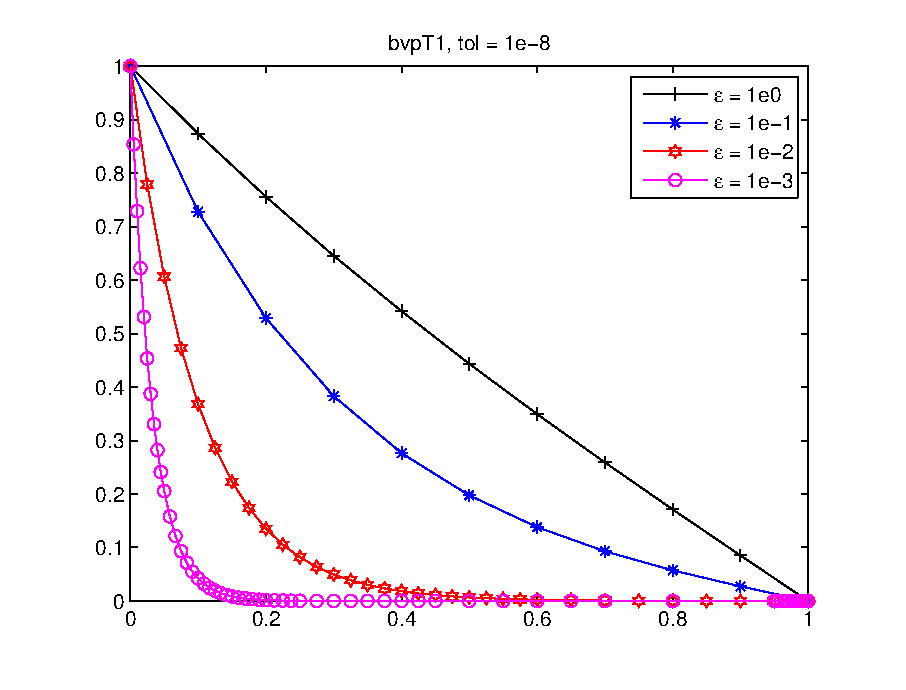
\includegraphics[height=6cm]{Prob1}}
\caption{Behavior of the solution of problem \ref{test1}.}
\end{figure}



\newpage
\subsection{Problem bvpT2}\label{test2}
The problem is 
\begin{equation*}
\begin{matrix}
\lambda z''  =  z', \quad z(0)=1, \quad z(1)=0,
\end{matrix}
\end{equation*}
with
\begin{equation*}
\begin{matrix}
z \in \mathbb{R}, \quad  t\in [0,1].
\end{matrix}
\end{equation*}
We write this problem in first order form by defining $y_1=z,$ and $y_2=z',$ yielding a system of differential equations of the form
\begin{equation*}
\begin{matrix}
\left(\begin{matrix}
y_1\\
y_2
\end{matrix}\right)'=
\left(\begin{matrix}
y_2\\
\frac{1}{\lambda}f(y_2)
\end{matrix}\right),
\end{matrix}
\end{equation*}
where
\begin{equation*}
\begin{matrix}
f(z')= z',
\end{matrix}
\end{equation*}
and
\begin{equation*}
\begin{matrix}
(y_1,y_2)^T \in \mathbb{R}^{2}, \quad  t \in [0,1].
\end{matrix}
\end{equation*}
The boundary conditions are obtained from
\begin{equation*}
\begin{matrix}
\left(
  \begin{matrix}
    1 & 0 \\
    0 & 0 \\
  \end{matrix}
\right)
\left(\begin{matrix}
y_{1}(0)\\
y_{2}(0)
\end{matrix}\right)
+
\left(
  \begin{matrix}
    0 & 0 \\
    1 & 0 \\
  \end{matrix}
\right)
\left(\begin{matrix}
y_{1}(1)\\
y_{2}(1)
\end{matrix}\right)=\left(\begin{matrix}
1 \\
0
\end{matrix}\right).
\end{matrix}
\end{equation*}
Exact solution
\begin{equation*}
\begin{matrix}
z(t) = (1 - \exp((t - 1) /\lambda)) / (1 - \exp(-1/\lambda)).
\end{matrix}
\end{equation*}
This problem is called \texttt{bvpT2} and we can solve
it by calling the driver function in command line as follows:
\begin{verbatim}
>> opts= bvptwpset('nmax',10000);
>> [sol,time]= bvpMtest(@bvpT2,'twpbvp_l',1e-4,1,opts,1e-3);
\end{verbatim}
\begin{figure}[htb]
\centerline{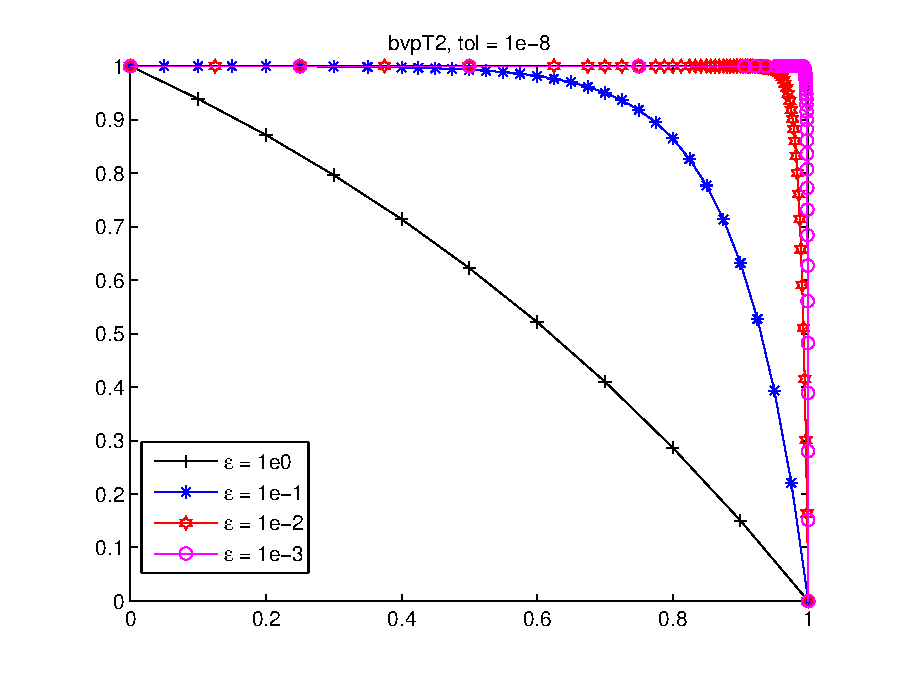
\includegraphics[height=6cm]{Prob2}}
\caption{Behavior of the solution of problem \ref{test2}.}
\end{figure}
\newpage
\subsection{Problem bvpT3}\label{test3}
The problem is 
\begin{eqnarray*}
\lambda z'' =  - (2 + \cos(\pi t)) z' + z  -(1 +\lambda \pi^{2}) \cos(\pi t) - (2 + \cos(\pi t)) \pi \sin(\pi t), \;\;\; z(-1)=-1 \;\;\; z(1)=-1,
\end{eqnarray*}
with
\[
z \in \RR, \;\;\; t\in [-1,1].
\]
We write this problem in first order form by defining $y_1=z$ and $y_2=z'$, yielding a system of
differential equations of the form
\begin{equation*}
\left(\begin{array}{c}
y_1\\
y_2
\end{array}\right)'=
\left(\begin{array}{c}
y_2\\
\frac{1}{\lambda}f(t,y_1,y_2)
\end{array}\right),
\end{equation*}
where
\begin{equation*}
 f(t,z,z') = - (2 + \cos(\pi t)) z' + z  -(1 +\lambda \pi^{2}) \cos(\pi t) - (2 + \cos(\pi t)) \pi \sin(\pi t),
\end{equation*}
and
\[
(y_1,y_2)^T \in \RR^{2}, \;\;\;  t \in [-1,1].
\]
The  boundary conditions are obtained from
\begin{equation*}
\left(
  \begin{array}{cc}
    1 & 0 \\
    0 & 0 \\
  \end{array}
\right)
\left(\begin{array}{c}
y_{1}(0)\\
y_{2}(0)
\end{array}\right)
+
\left(
  \begin{array}{cc}
    0 & 0 \\
    1 & 0 \\
  \end{array}
\right)
\left(\begin{array}{c}
y_{1}(1)\\
y_{2}(1)
\end{array}\right)=\left(\begin{array}{c}
-1 \\
-1
\end{array}\right).
\end{equation*}
\textrm{Exact solution}
$$z(t) = \cos(\pi t).$$
The problem has no turning points and the solution is smooth.
\begin{figure}[htb]
\centerline{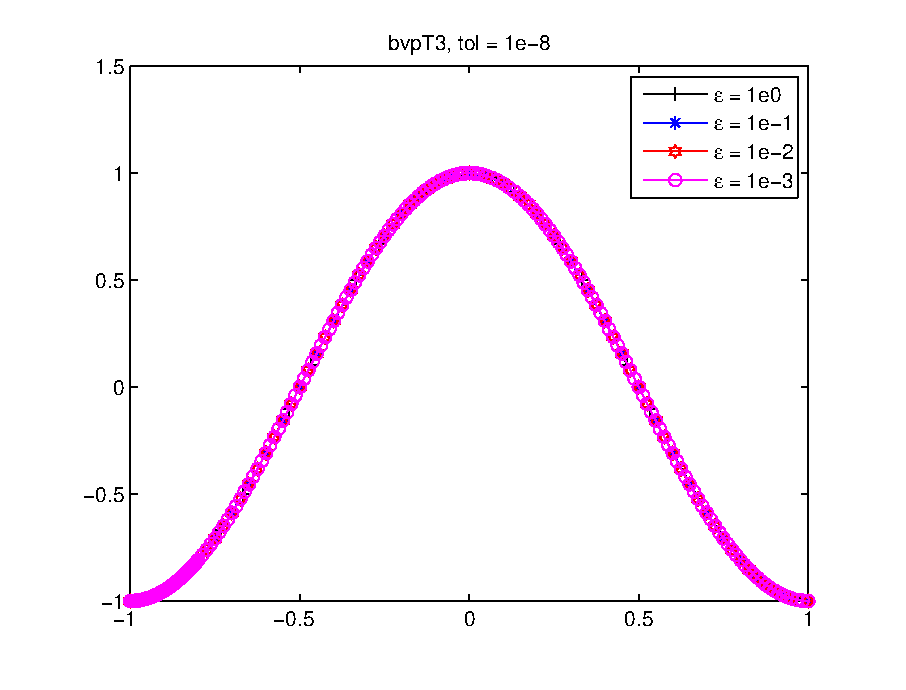
\includegraphics[height=6cm]{Prob3}}
\caption{Behavior of the solution of problem \ref{test3}.}
\end{figure}
\newpage
\subsection{Problem bvpT4}\label{test4}
The problem is
\begin{eqnarray*}
\lambda z'' = - z' + (1 +\lambda) z, \;\;\; z(-1) = 1 + \exp(-2), \;\;\; z(1) = 1 + \exp(-2(1+\lambda)/\lambda),
\end{eqnarray*}
with
\[
z \in \RR, \;\;\; t\in [-1,1].
\]
We write this problem in first order form by defining $y_1=z$ and $y_2=z'$, yielding a system of differential equations of the form
\begin{equation*}
\left(\begin{array}{c}
y_1\\
y_2
\end{array}\right)'=
\left(\begin{array}{c}
y_2\\
\frac{1}{\lambda}f(y_1,y_2)
\end{array}\right),
\end{equation*}
where
\begin{equation*}
f(z,z') = -z' + (1 +\lambda) z,
\end{equation*}
and
\[
(y_1,y_2)^T \in \RR^{2}, \;\;\;  t \in [-1,1].
\]
The  boundary conditions are obtained from
\begin{equation*}
\left(
  \begin{array}{cc}
    1 & 0 \\
    0 & 0 \\
  \end{array}
\right)
\left(\begin{array}{c}
y_{1}(0)\\
y_{2}(0)
\end{array}\right)
+
\left(
  \begin{array}{cc}
    0 & 0 \\
    1 & 0 \\
  \end{array}
\right)
\left(\begin{array}{c}
y_{1}(1)\\
y_{2}(1)
\end{array}\right)=\left(\begin{array}{c}
1 + \exp(-2) \\
1 + \exp(-2(1+\lambda)/\lambda)
\end{array}\right).
\end{equation*}
\textrm{Exact solution}
$$z(t) = \exp(t -1) + \exp(-(1 +\lambda)(1 +t) /\lambda).$$
The solution has a boundary layer of width $O(\epsilon)$  at $t = -1.$
\begin{figure}[htb]
\centerline{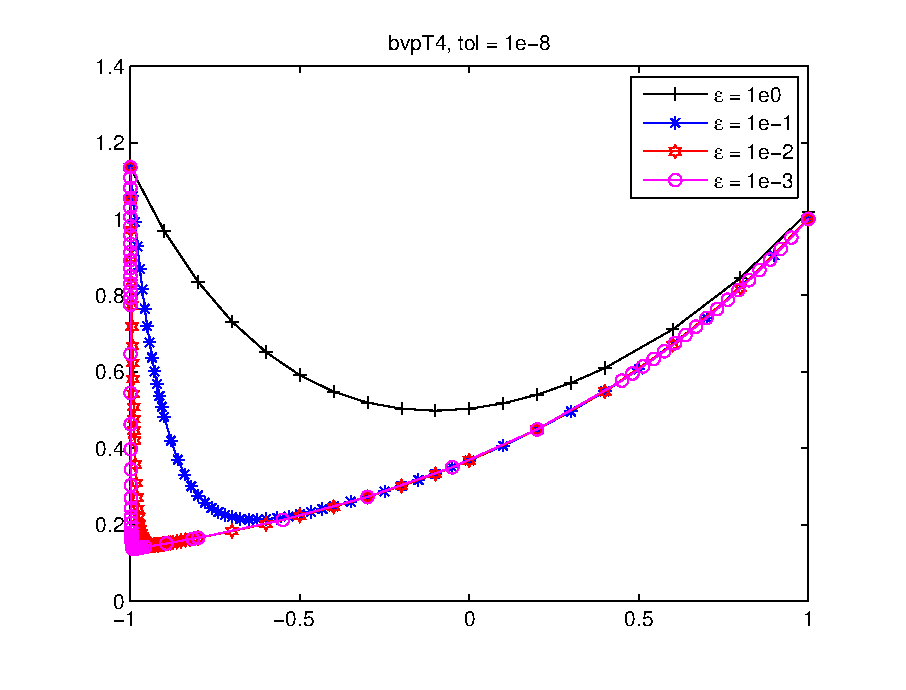
\includegraphics[height=6cm]{Prob4}}
\caption{Behavior of the solution of problem \ref{test4}.}
\end{figure}
\newpage
\subsection{Problem bvpT5}\label{test5}
The problem is 
\begin{eqnarray*}
\lambda z'' =  t z' + z -( 1 +\lambda \pi^{2}) \cos(\pi t) + \pi t \sin(\pi t), \;\;\;z(-1) =   -1, \;\;\; z(1) = -1,
\end{eqnarray*}
with
\[
z \in \RR, \;\;\; t\in [-1,1].
\]
We write this problem in first order form by defining $y_1=z$ and $y_2=z'$, yielding a system of differential equations of the form
\begin{equation*}
\left(\begin{array}{c}
y_1\\
y_2
\end{array}\right)'=
\left(\begin{array}{c}
y_2\\
\frac{1}{\lambda}f(t,y_1,y_2)
\end{array}\right),
\end{equation*}
where
\begin{equation*}
f(t,z,z') = t z' + z -( 1 +\lambda \pi^{2}) \cos(\pi t) + \pi t \sin(\pi t),
\end{equation*}
and
\[
(y_1,y_2)^T \in \RR^{2}, \;\;\;  t \in [-1,1].
\]
The  boundary conditions are obtained from
\begin{equation*}
\left(
  \begin{array}{cc}
    1 & 0 \\
    0 & 0 \\
  \end{array}
\right)
\left(\begin{array}{c}
y_{1}(0)\\
y_{2}(0)
\end{array}\right)
+
\left(
  \begin{array}{cc}
    0 & 0 \\
    1 & 0 \\
  \end{array}
\right)
\left(\begin{array}{c}
y_{1}(1)\\
y_{2}(1)
\end{array}\right)=\left(\begin{array}{c}
-1 \\
-1
\end{array}\right).
\end{equation*}
\textrm{Exact solution}
$$z(t) = \cos(\pi t).$$
The problem has a turning point at $t=0$ but the solution is smooth.

\begin{figure}[htb]
\centerline{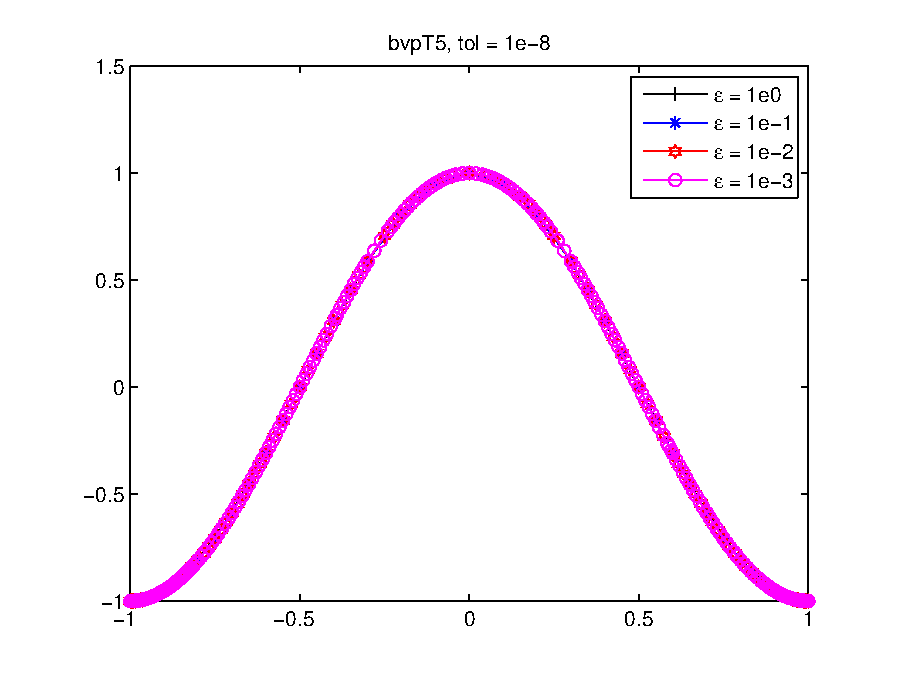
\includegraphics[height=6cm]{Prob5}}
\caption{Behavior of the solution of problem \ref{test5}.}
\end{figure}
\newpage
\subsection{Problem bvpT6}\label{test6}
The problem is 
\begin{eqnarray*}
\lambda z'' = - t z'  -\lambda \pi^{2} \cos(\pi t) - \pi t \sin(\pi t), \;\;\;z(-1) =   -2, \;\;\; z(1) = 0,
\end{eqnarray*}
with
\[
z \in \RR, \;\;\; t\in [-1,1].
\]
We write this problem in first order form by defining $y_1=z$ and $y_2=z'$, yielding a system of differential equations of the form
\begin{equation*}
\left(\begin{array}{c}
y_1\\
y_2
\end{array}\right)'=
\left(\begin{array}{c}
y_2\\
\frac{1}{\lambda}f(t,y_2)
\end{array}\right),
\end{equation*}
where
\begin{equation*}
f(t,z') = - t z'  -\lambda \pi^{2} \cos(\pi t) - \pi t \sin(\pi t),
\end{equation*}
with
\[
(y_1,y_2)^T \in \RR^{2}, \;\;\;  t \in [-1,1].
\]
The  boundary conditions are obtained from
\begin{equation*}
\left(
  \begin{array}{cc}
    1 & 0 \\
    0 & 0 \\
  \end{array}
\right)
\left(\begin{array}{c}
y_{1}(0)\\
y_{2}(0)
\end{array}\right)
+
\left(
  \begin{array}{cc}
    0 & 0 \\
    1 & 0 \\
  \end{array}
\right)
\left(\begin{array}{c}
y_{1}(1)\\
y_{2}(1)
\end{array}\right)=\left(\begin{array}{c}
-2 \\
0
\end{array}\right).
\end{equation*}
\textrm{Exact solution}
$$z(t) = \cos(\pi t) +  \textmd{erf}(t / \sqrt{ 2\lambda}) /  \textmd{erf}(1 / \sqrt{2\lambda}).$$
The solution has a shock layer in the turning point region near $t =0.$

\begin{figure}[htb]
\centerline{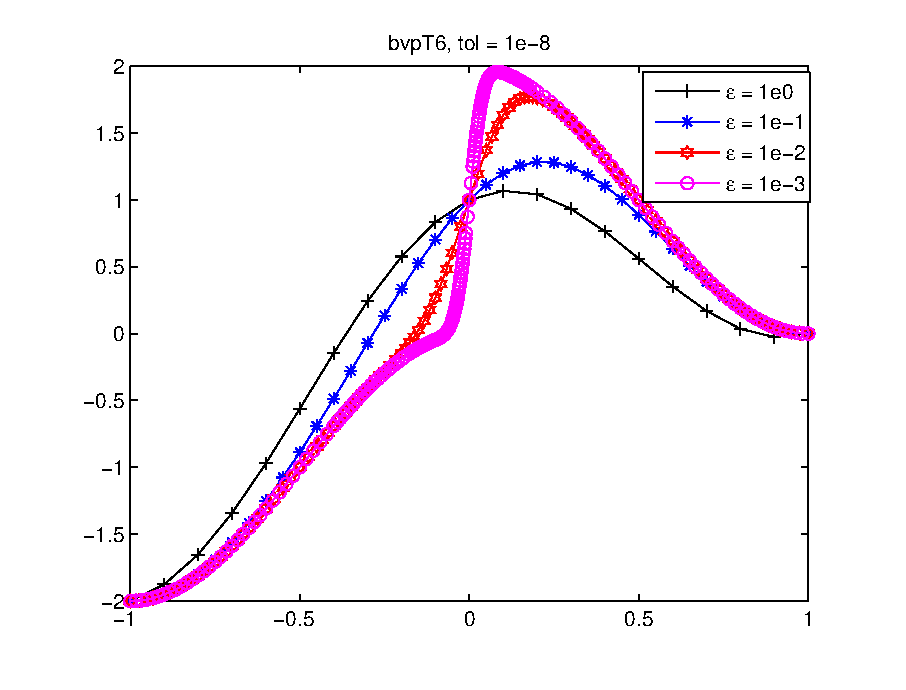
\includegraphics[height=6cm]{Prob6}}
\caption{Behavior of the solution of problem \ref{test6}.}
\end{figure}
\newpage
\subsection{Problem bvpT7}\label{test7}
The problem is 
\begin{eqnarray*}
\lambda z'' = - t z' + z - (1 +\lambda \pi^{2}) \cos(\pi t) - \pi t \sin(\pi t), \;\;\;z(-1) =   -1, \;\;\; z(1) = 1,
\end{eqnarray*}
with
\[
z \in \RR, \;\;\; t\in [-1,1].
\]
We write this problem in first order form by defining $y_1=z$ and $y_2=z'$, yielding a system of differential equations of the form
\begin{equation*}
\left(\begin{array}{c}
y_1\\
y_2
\end{array}\right)'=
\left(\begin{array}{c}
y_2\\
\frac{1}{\lambda}f(t,y_1,y_2)
\end{array}\right),
\end{equation*}
where
\begin{equation*}
  f(t,z,z') = - t z' + z - (1 +\lambda \pi^{2}) \cos(\pi t) - \pi t \sin(\pi t),
\end{equation*}
with
\[
(y_1,y_2)^T \in \RR^{2}, \;\;\;  t \in [-1,1].
\]
The  boundary conditions are obtained from
\begin{equation*}
\left(
  \begin{array}{cc}
    1 & 0 \\
    0 & 0 \\
  \end{array}
\right)
\left(\begin{array}{c}
y_{1}(0)\\
y_{2}(0)
\end{array}\right)
+
\left(
  \begin{array}{cc}
    0 & 0 \\
    1 & 0 \\
  \end{array}
\right)
\left(\begin{array}{c}
y_{1}(1)\\
y_{2}(1)
\end{array}\right)=\left(\begin{array}{c}
-1 \\
1
\end{array}\right).
\end{equation*}
\textrm{Exact solution}
$$z(t) =  \cos(\pi t) +  t + \frac{ \displaystyle{t \, \textmd{erf}(t / \sqrt{2\lambda}) + \sqrt{2\lambda / \pi} \exp(-t^{2} / 2\lambda)}}
{\displaystyle{\textmd{erf}(1 / \sqrt{2\lambda}) + \sqrt{2\lambda / \pi} \exp(-1 / 2\lambda)}}.$$
The solution has a corner layer in the turning point region near $t =0.$

\begin{figure}[htb]
\centerline{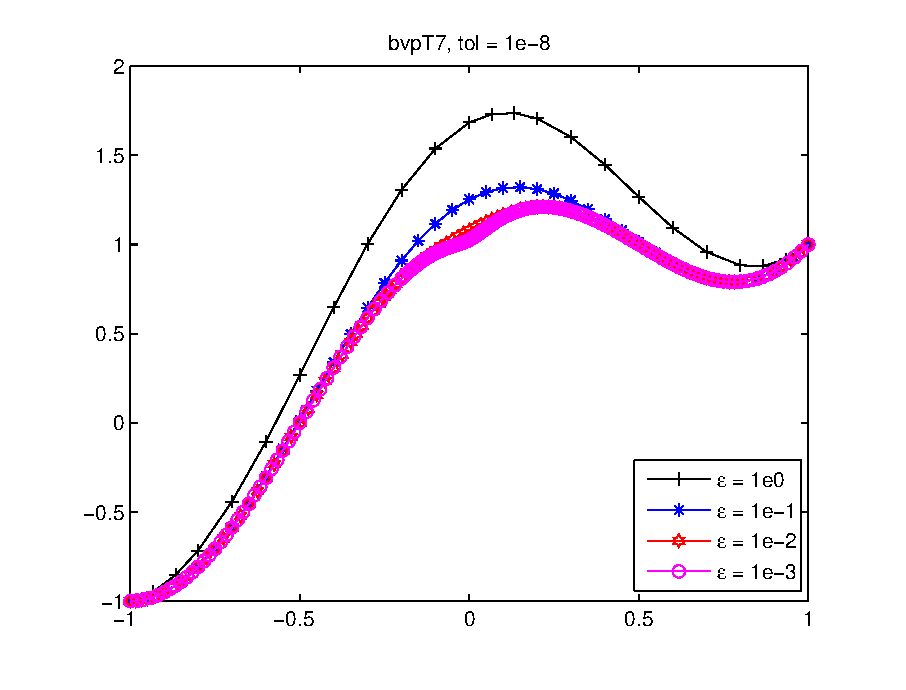
\includegraphics[height=6cm]{Prob7}}
\caption{Behavior of the solution of problem \ref{test7}.}
\end{figure}
\newpage
\subsection{Problem bvpT8}\label{test8}
The problem is 
\begin{eqnarray*}
\lambda z'' = -z', \;\;\;z(0) =   1, \;\;\; z(1) = 2,
\end{eqnarray*}
with
\[
z \in \RR, \;\;\; t\in [0,1].
\]
We write this problem in first order form by defining $y_1=z$ and $y_2=z'$, yielding a system of differential equations of the form
\begin{equation*}
\left(\begin{array}{c}
y_1\\
y_2
\end{array}\right)'=
\left(\begin{array}{c}
y_2\\
\frac{1}{\lambda}f(y_2)
\end{array}\right),
\end{equation*}
where
\begin{equation*}
f(z') = -z',
\end{equation*}
with
\[
(y_1,y_2)^T \in \RR^{2}, \;\;\;  t \in [0,1].
\]
The  boundary conditions are obtained from
\begin{equation*}
\left(
  \begin{array}{cc}
    1 & 0 \\
    0 & 0 \\
  \end{array}
\right)
\left(\begin{array}{c}
y_{1}(0)\\
y_{2}(0)
\end{array}\right)
+
\left(
  \begin{array}{cc}
    0 & 0 \\
    1 & 0 \\
  \end{array}
\right)
\left(\begin{array}{c}
y_{1}(1)\\
y_{2}(1)
\end{array}\right)=\left(\begin{array}{c}
1 \\
2
\end{array}\right).
\end{equation*}
\textrm{Exact solution}
$$z(t) =  (2 - \exp(-1/\lambda) - \exp(-t /\lambda)) / (1 - \exp(-1 /\lambda)).$$
The solution has a boundary layer of width $O(\lambda)$  at $t = 0.$

\begin{figure}[htb]
\centerline{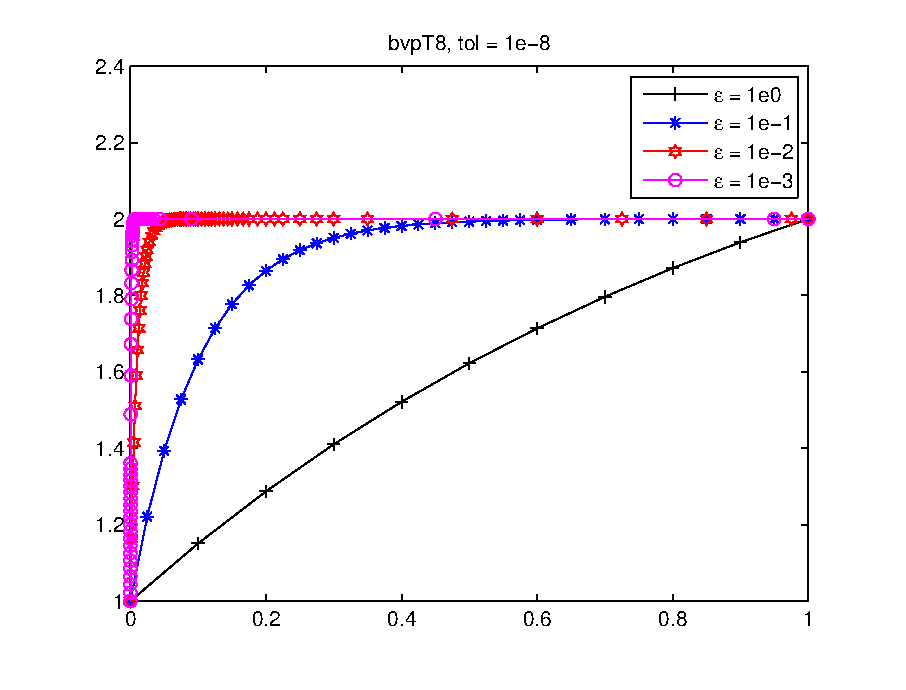
\includegraphics[height=6cm]{Prob8}}
\caption{Behavior of the solution of problem \ref{test8}.}
\end{figure}
\newpage
\subsection{Problem bvpT9}\label{test9}
The problem is 
\begin{eqnarray*}
(\lambda + t^{2})z'' = -4tz' - 2z, \;\;\;z(-1) = 1 / (1 +\lambda), \;\;\; z(1) = 1 / (1 +\lambda),
\end{eqnarray*}
with
\[
z \in \RR, \;\;\; t\in [-1,1].
\]
We write this problem in first order form by defining $y_1=z$ and $y_2=z'$, yielding a system of differential equations of the form
\begin{equation*}
\left(\begin{array}{c}
y_1\\
y_2
\end{array}\right)'=
\left(\begin{array}{c}
y_2\\
\frac{1}{\lambda+ t^{2}}f(t,y_1,y_2)
\end{array}\right),
\end{equation*}
where
\begin{equation*}
 f(t,z,z') = -4tz' - 2z,
\end{equation*}
with
\[
(y_1,y_2)^T \in \RR^{2}, \;\;\;  t \in [-1,1].
\]
The  boundary conditions are obtained from
\begin{equation*}
\left(
  \begin{array}{cc}
    1 & 0 \\
    0 & 0 \\
  \end{array}
\right)
\left(\begin{array}{c}
y_{1}(0)\\
y_{2}(0)
\end{array}\right)
+
\left(
  \begin{array}{cc}
    0 & 0 \\
    1 & 0 \\
  \end{array}
\right)
\left(\begin{array}{c}
y_{1}(1)\\
y_{2}(1)
\end{array}\right)=\left(\begin{array}{c}
1 / (1 +\lambda) \\
1 / (1 +\lambda)
\end{array}\right).
\end{equation*}
\textrm{Exact solution}
$$z(t) = 1 / (\lambda + x^{2}).$$
The solution has a spike of height $\frac{1}{\lambda}$ at $t = 0.$

\begin{figure}[htb]
\centerline{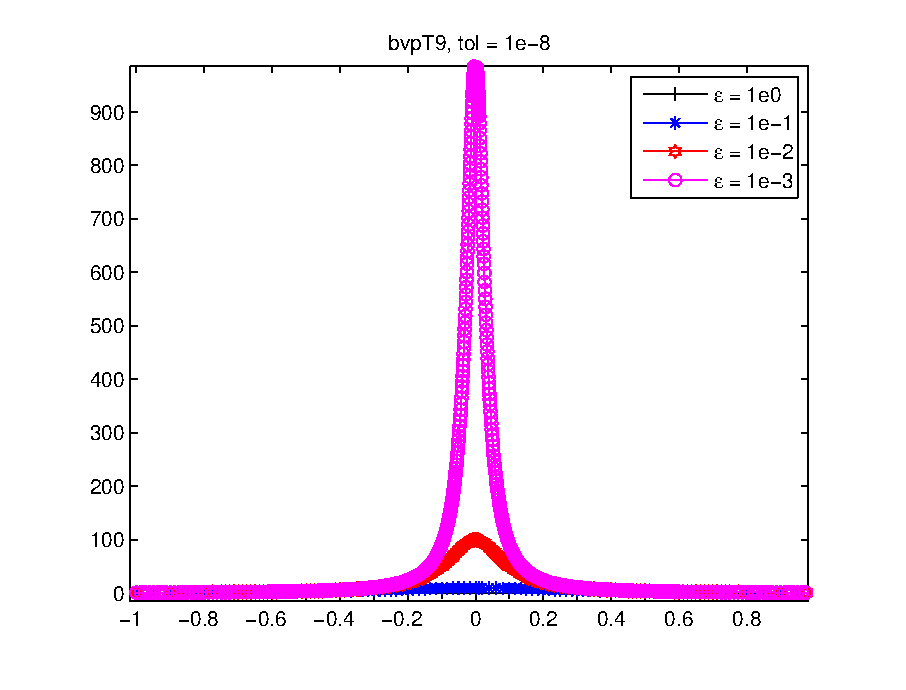
\includegraphics[height=6cm]{Prob9}}
\caption{Behavior of the solution of problem \ref{test9}.}
\end{figure}
\newpage
\subsection{Problem bvpT10}\label{test10}
The problem is 
\begin{eqnarray*}
\lambda z'' = -t z' , \;\;\;z(-1) = 0, \;\;\; z(1) = 2,
\end{eqnarray*}
with
\[
z \in \RR, \;\;\; t\in [-1,1].
\]
We write this problem in first order form by defining $y_1=z$ and $y_2=z'$, yielding a system of differential equations of the form
\begin{equation*}
\left(\begin{array}{c}
y_1\\
y_2
\end{array}\right)'=
\left(\begin{array}{c}
y_2\\
\frac{1}{\lambda}f(t,y_2)
\end{array}\right),
\end{equation*}
where
\begin{equation*}
 f(t,z') = -t z',
\end{equation*}
with
\[
(y_1,y_2)^T \in \RR^{2}, \;\;\;  t \in [-1,1].
\]
The  boundary conditions are obtained from
\begin{equation*}
\left(
  \begin{array}{cc}
    1 & 0 \\
    0 & 0 \\
  \end{array}
\right)
\left(\begin{array}{c}
y_{1}(0)\\
y_{2}(0)
\end{array}\right)
+
\left(
  \begin{array}{cc}
    0 & 0 \\
    1 & 0 \\
  \end{array}
\right)
\left(\begin{array}{c}
y_{1}(1)\\
y_{2}(1)
\end{array}\right)=\left(\begin{array}{c}
0 \\
2
\end{array}\right).
\end{equation*}
\textrm{Exact solution}
$$z(t) = 1 + \textmd{erf}(t / \sqrt{2\lambda}) / \textmd{erf}(1 / \sqrt{2\lambda}).$$
The solution has a turning point of width $O(\sqrt\lambda)$  at $t = 0.$

\begin{figure}[htb]
\centerline{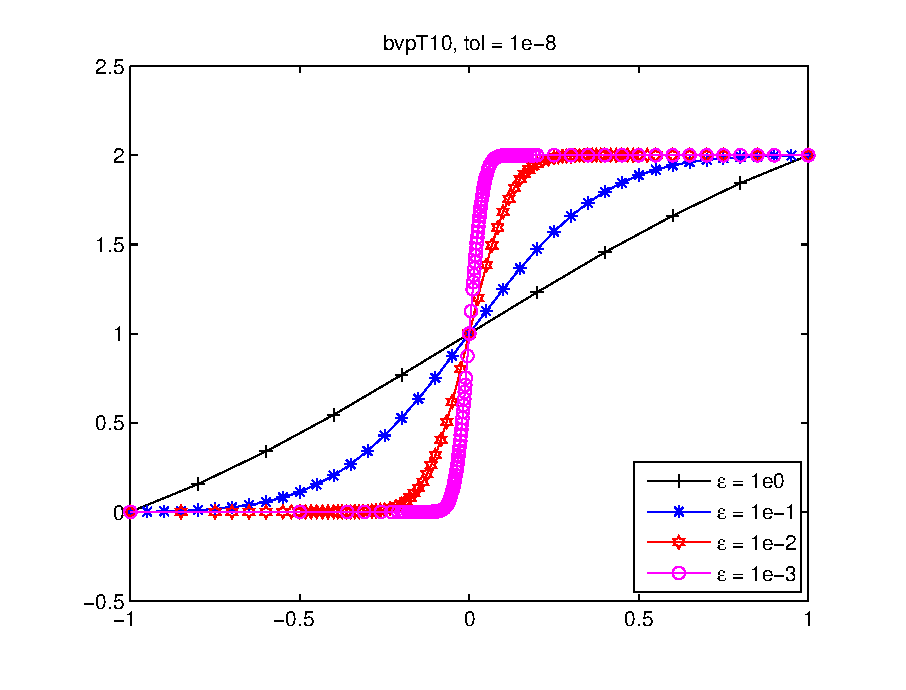
\includegraphics[height=6cm]{Prob10}}
\caption{Behavior of the solution of problem \ref{test10}.}
\end{figure}
\newpage
\subsection{Problem bvpT11}\label{test11}
The problem is 
\begin{eqnarray*}
\lambda z'' =  z -(1 +\lambda \pi^{2}) \cos(\pi t), \;\;\;z(-1) = -1, \;\;\; z(1) = -1,
\end{eqnarray*}
with
\[
z \in \RR, \;\;\; t\in [-1,1].
\]
We write this problem in first order form by defining $y_1=z$ and $y_2=z'$, yielding a system of differential equations of the form
\begin{equation*}
\left(\begin{array}{c}
y_1\\
y_2
\end{array}\right)'=
\left(\begin{array}{c}
y_2\\
\frac{1}{\lambda}f(t,y_1)
\end{array}\right),
\end{equation*}
where
\begin{equation*}
f(t,z) =  z -(1 +\lambda \pi^{2}) \cos(\pi t),
\end{equation*}
with
\[
(y_1,y_2)^T \in \RR^{2}, \;\;\;  t \in [-1,1].
\]
The  boundary conditions are obtained from
\begin{equation*}
\left(
  \begin{array}{cc}
    1 & 0 \\
    0 & 0 \\
  \end{array}
\right)
\left(\begin{array}{c}
y_{1}(0)\\
y_{2}(0)
\end{array}\right)
+
\left(
  \begin{array}{cc}
    0 & 0 \\
    1 & 0 \\
  \end{array}
\right)
\left(\begin{array}{c}
y_{1}(1)\\
y_{2}(1)
\end{array}\right)=\left(\begin{array}{c}
-1 \\
-1
\end{array}\right).
\end{equation*}
\textrm{Exact solution}
$$z(t) = \cos(\pi t).$$
The solution is smooth.

\begin{figure}[htb]
\centerline{\includegraphics[height=6cm]{Prob11}}
\caption{Behavior of the solution of problem \ref{test11}.}
\end{figure}
\newpage
\subsection{Problem bvpT12}\label{test12}
The problem is 
\begin{eqnarray*}
\lambda z'' =  z  - (1 +\lambda \pi^{2}) \cos(\pi t), \;\;\;z(-1) = -1, \;\;\; z(1) = 0,
\end{eqnarray*}
with
\[
z \in \RR, \;\;\; t\in [-1,1].
\]
We write this problem in first order form by defining $y_1=z$ and $y_2=z'$, yielding a system of differential equations of the form
\begin{equation*}
\left(\begin{array}{c}
y_1\\
y_2
\end{array}\right)'=
\left(\begin{array}{c}
y_2\\
\frac{1}{\lambda}f(t,y_1)
\end{array}\right),
\end{equation*}
where
\begin{equation*}
f(t,z) = z  - (1 +\lambda \pi^{2}) \cos(\pi t),
\end{equation*}
with
\[
(y_1,y_2)^T \in \RR^{2}, \;\;\;  t \in [-1,1].
\]
The  boundary conditions are obtained from
\begin{equation*}
\left(
  \begin{array}{cc}
    1 & 0 \\
    0 & 0 \\
  \end{array}
\right)
\left(\begin{array}{c}
y_{1}(0)\\
y_{2}(0)
\end{array}\right)
+
\left(
  \begin{array}{cc}
    0 & 0 \\
    1 & 0 \\
  \end{array}
\right)
\left(\begin{array}{c}
y_{1}(1)\\
y_{2}(1)
\end{array}\right)=\left(\begin{array}{c}
-1 \\
0
\end{array}\right).
\end{equation*}
\textrm{Exact solution}
$$z(t) = \cos(\pi t) +  \frac{\displaystyle{\exp((t + 1) / \sqrt\lambda) - \exp((-t -1) / \sqrt\lambda)}}
{\displaystyle{\exp(2 / \sqrt\lambda) - \exp(-2 / \sqrt\lambda)}}.$$
The solution has a turning point of width $O(\sqrt\lambda)$  at $t = 1.$

\begin{figure}[htb]
\centerline{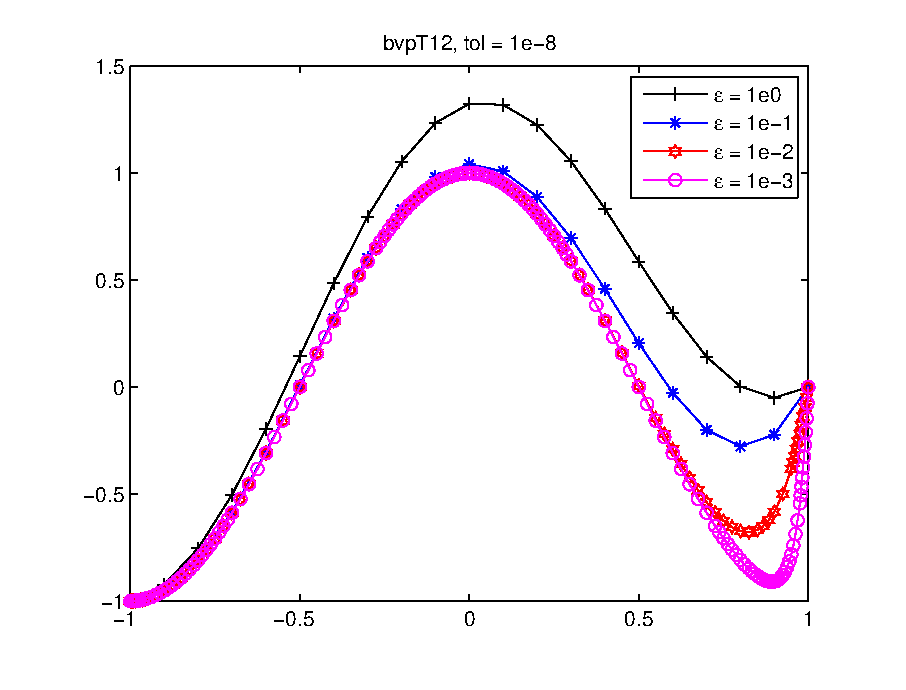
\includegraphics[height=6cm]{Prob12}}
\caption{Behavior of the solution of problem \ref{test12}.}
\end{figure}
\newpage
\subsection{Problem bvpT13}\label{test13}
The problem is
\begin{eqnarray*}
\lambda z'' =  z  - (1 +\lambda \pi^{2}) \cos(\pi t), \;\;\;z(-1) = 0, \;\;\; z(1) = 1,
\end{eqnarray*}
with
\[
z \in \RR, \;\;\; t\in [-1,1].
\]
We write this problem in first order form by defining $y_1=z$ and $y_2=z'$, yielding a system of differential equations of the form
\begin{equation*}
\left(\begin{array}{c}
y_1\\
y_2
\end{array}\right)'=
\left(\begin{array}{c}
y_2\\
\frac{1}{\lambda}f(t,y_1)
\end{array}\right),
\end{equation*}
where
\begin{equation*}
 f(t,z) = z  - (1 +\lambda \pi^{2}) \cos(\pi t).
\end{equation*}
with
\[
(y_1,y_2)^T \in \RR^{2}, \;\;\;  t \in [-1,1].
\]
The  boundary conditions are obtained from
\begin{equation*}
\left(
  \begin{array}{cc}
    1 & 0 \\
    0 & 0 \\
  \end{array}
\right)
\left(\begin{array}{c}
y_{1}(0)\\
y_{2}(0)
\end{array}\right)
+
\left(
  \begin{array}{cc}
    0 & 0 \\
    1 & 0 \\
  \end{array}
\right)
\left(\begin{array}{c}
y_{1}(1)\\
y_{2}(1)
\end{array}\right)=\left(\begin{array}{c}
0 \\
-1
\end{array}\right).
\end{equation*}
\textrm{Exact solution}
$$z(t) = \cos(\pi t) +  \exp(-(t + 1) / \sqrt\lambda).$$
The solution has a boundary layer of width $O(\sqrt\lambda)$ near $t = -1.$

\begin{figure}[htb]
\centerline{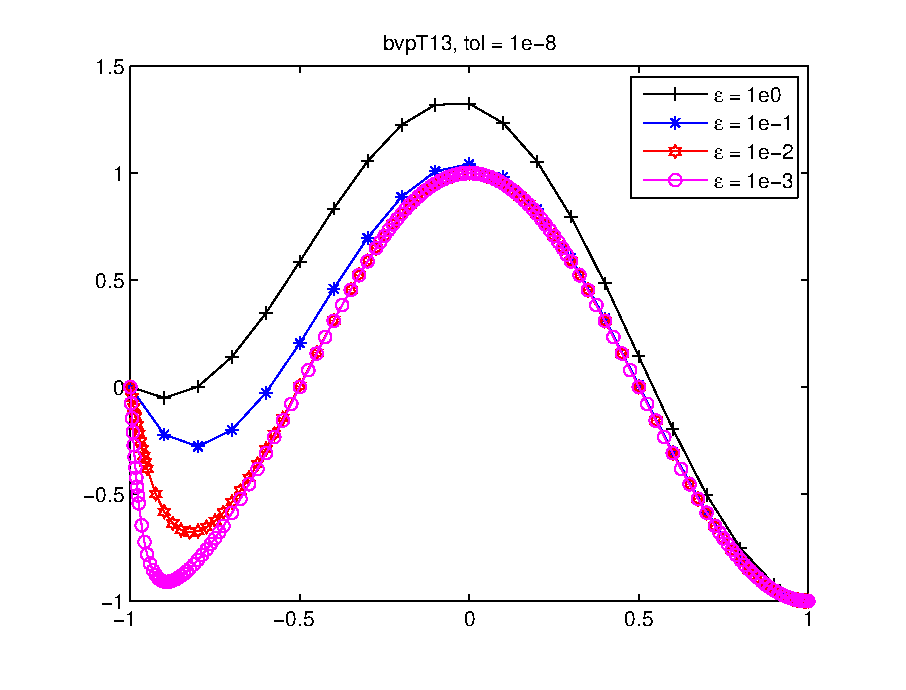
\includegraphics[height=6cm]{Prob13}}
\caption{Behavior of the solution of problem \ref{test13}.}
\end{figure}
 \newpage
\subsection{Problem bvpT14}\label{test14}
The problem is 
\begin{eqnarray*}
\lambda z'' = z  - (1 +\lambda \pi^{2}) \cos(\pi t), \;\;\;z(-1) = 0, \;\;\; z(1) = 0,
\end{eqnarray*}
with
\[
z \in \RR, \;\;\; t\in [-1,1].
\]
We write this problem in first order form by defining $y_1=z$ and $y_2=z'$, yielding a system of differential equations of the form
\begin{equation*}
\left(\begin{array}{c}
y_1\\
y_2
\end{array}\right)'=
\left(\begin{array}{c}
y_2\\
\frac{1}{\lambda}f(t,y_1)
\end{array}\right),
\end{equation*}
where
\begin{equation*}
 f(t,z) = z  - (1 +\lambda \pi^{2}) \cos(\pi t),
\end{equation*}
with
\[
(y_1,y_2)^T \in \RR^{2}, \;\;\;  t \in [-1,1].
\]
The  boundary conditions are obtained from
\begin{equation*}
\left(
  \begin{array}{cc}
    1 & 0 \\
    0 & 0 \\
  \end{array}
\right)
\left(\begin{array}{c}
y_{1}(0)\\
y_{2}(0)
\end{array}\right)
+
\left(
  \begin{array}{cc}
    0 & 0 \\
    1 & 0 \\
  \end{array}
\right)
\left(\begin{array}{c}
y_{1}(1)\\
y_{2}(1)
\end{array}\right)=\left(\begin{array}{c}
0 \\
0
\end{array}\right).
\end{equation*}
\textrm{Exact solution}
$$z(t) =  \cos(\pi t) +  \exp((t - 1) / \sqrt\lambda) + \exp(-(t + 1) / \sqrt\lambda).$$
The solution has a boundary layer of width $O(\sqrt\lambda)$  near $t = -1$ and $t = 1.$

\begin{figure}[htb]
\centerline{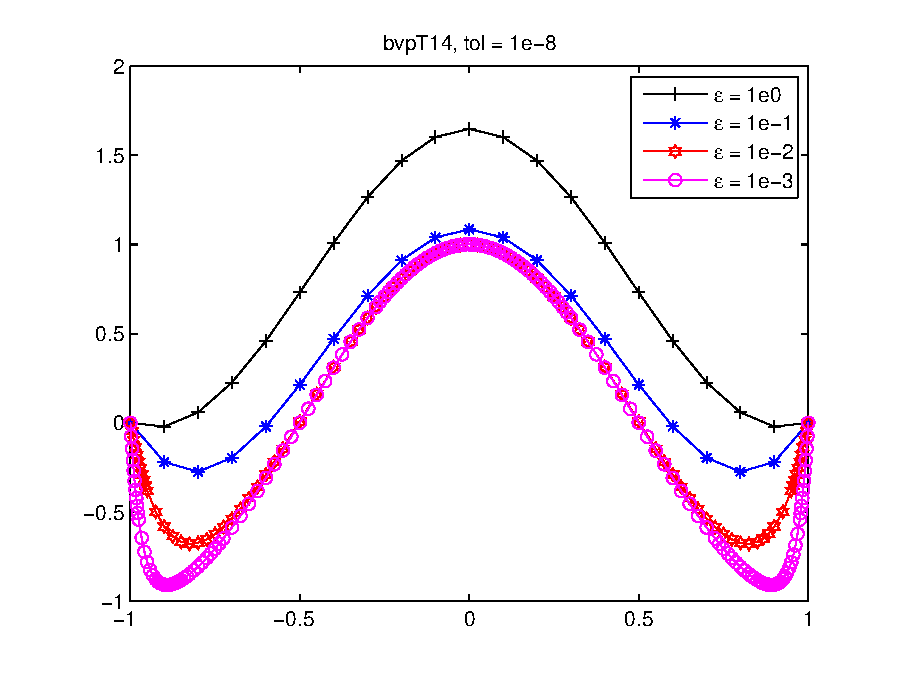
\includegraphics[height=6cm]{Prob14}}
\caption{Behavior of the solution of problem \ref{test14}.}
\end{figure}
\newpage
\subsection{Problem bvpT15}\label{test15}
The problem is 
\begin{eqnarray*}
\lambda z'' = t z, \;\;\;z(-1) = 1, \;\;\; z(1) = 1,
\end{eqnarray*}
with
\[
z \in \RR, \;\;\; t\in [-1,1].
\]
We write this problem in first order form by defining $y_1=z$ and $y_2=z'$, yielding a system of differential equations of the form
\begin{equation*}
\left(\begin{array}{c}
y_1\\
y_2
\end{array}\right)'=
\left(\begin{array}{c}
y_2\\
\frac{1}{\lambda}f(t,y_1)
\end{array}\right),
\end{equation*}
where
\begin{equation*}
 f(t,z) = t z,
\end{equation*}
with
\[
(y_1,y_2)^T \in \RR^{2}, \;\;\;  t \in [-1,1].
\]
The  boundary conditions are obtained from
\begin{equation*}
\left(
  \begin{array}{cc}
    1 & 0 \\
    0 & 0 \\
  \end{array}
\right)
\left(\begin{array}{c}
y_{1}(0)\\
y_{2}(0)
\end{array}\right)
+
\left(
  \begin{array}{cc}
    0 & 0 \\
    1 & 0 \\
  \end{array}
\right)
\left(\begin{array}{c}
y_{1}(1)\\
y_{2}(1)
\end{array}\right)=\left(\begin{array}{c}
1 \\
1
\end{array}\right).
\end{equation*}

\begin{figure}[htb]
\centerline{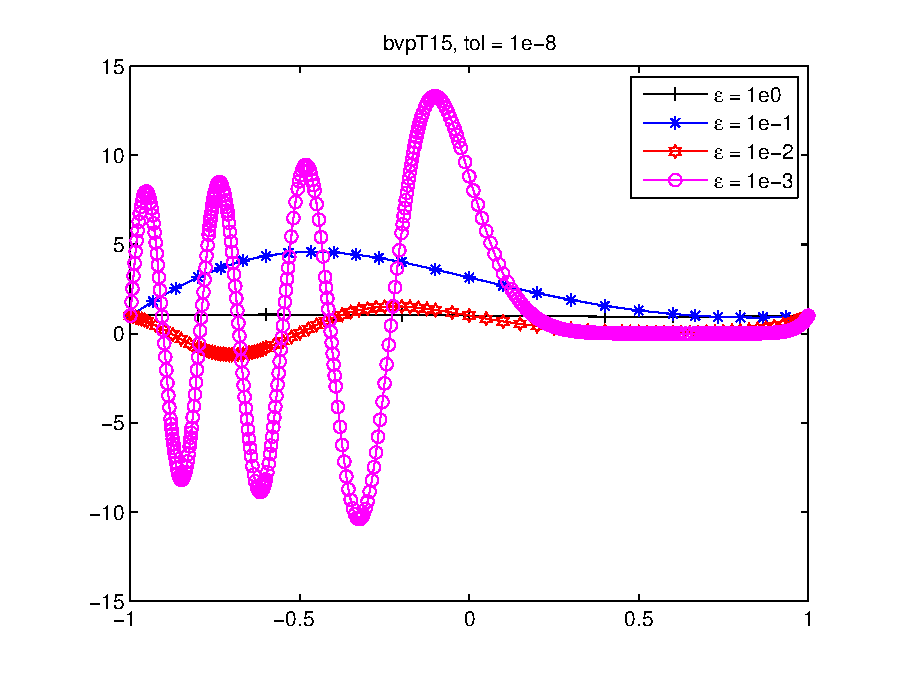
\includegraphics[height=6cm]{Prob15}}
\caption{Behavior of the solution of problem \ref{test15}.}
\end{figure}
\newpage
\subsection{Problem bvpT16}\label{test16}
The problem is 
\begin{eqnarray*}
\lambda^{2} z'' = -\pi^{2} z / 4, \;\;\;z(0) = \sin(\pi / 2\lambda), \;\;\; z(1) = \sin(\pi / 2\lambda),
\end{eqnarray*}
with
\[
z \in \RR, \;\;\; t\in [0,1].
\]
We write this problem in first order form by defining $y_1=z$ and $y_2=z'$, yielding a system of differential equations of the form
\begin{equation*}
\left(\begin{array}{c}
y_1\\
y_2
\end{array}\right)'=
\left(\begin{array}{c}
y_2\\
\frac{1}{\lambda^{2}}f(y_1)
\end{array}\right),
\end{equation*}
where
\begin{equation*}
f(z) = -\pi^{2} z / 4,
\end{equation*}
with
\[
(y_1,y_2)^T \in \RR^{2}, \;\;\;  t \in [0,1].
\]
The  boundary conditions are obtained from
\begin{equation*}
\left(
  \begin{array}{cc}
    1 & 0 \\
    0 & 0 \\
  \end{array}
\right)
\left(\begin{array}{c}
y_{1}(0)\\
y_{2}(0)
\end{array}\right)
+
\left(
  \begin{array}{cc}
    0 & 0 \\
    1 & 0 \\
  \end{array}
\right)
\left(\begin{array}{c}
y_{1}(1)\\
y_{2}(1)
\end{array}\right)=\left(\begin{array}{c}
\sin(\pi / 2\lambda) \\
\sin(\pi / 2\lambda)
\end{array}\right).
\end{equation*}
\textrm{Exact solution}
$$z(t) =  \sin( \pi t / 2\lambda) \operatorname{when} 1/\lambda \operatorname{is odd}.$$
The solution oscillates rapidly for small $\lambda.$

\begin{figure}[htb]
\centerline{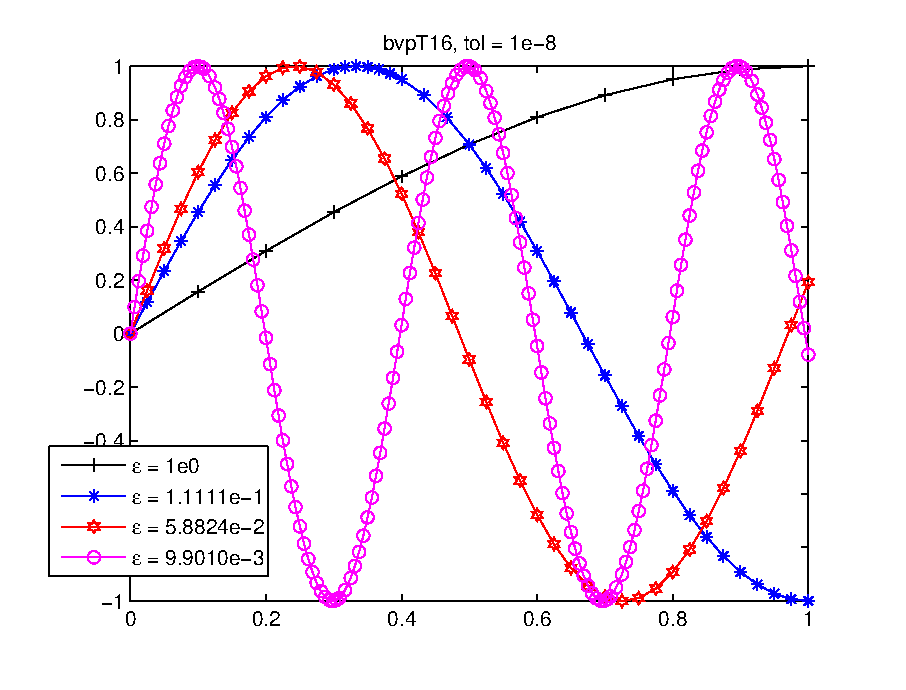
\includegraphics[height=6cm]{Prob16}}
\caption{Behavior of the solution of problem \ref{test16}.}
\end{figure}
\newpage
\subsection{Problem bvpT17}\label{test17}
The problem is 
\begin{eqnarray*}
 z'' =  -3\lambda z / (\epsilon + t^{2})^{2}, \;\;\;z(-0.1) = -0.1 / \sqrt{\lambda + 0.01}, \;\;\; z(0.1) = 0.1 / \sqrt{\lambda + 0.01}
\end{eqnarray*}
with
\[
z \in \RR, \;\;\; t\in [-0.1,0.1].
\]
We write this problem in first order form by defining $y_1=z$ and $y_2=z'$, yielding a system of differential equations of the form
\begin{equation*}
\left(\begin{array}{c}
y_1\\
y_2
\end{array}\right)'=
\left(\begin{array}{c}
y_2\\
f(t,y_1)
\end{array}\right),
\end{equation*}
where
\begin{equation*}
f(t,z) = -3\lambda z / (\lambda + t^{2})^{2},
\end{equation*}
with
\[
(y_1,y_2)^T \in \RR^{2}, \;\;\;  t \in [-0.1,0.1].
\]
The  boundary conditions are obtained from
\begin{equation*}
\left(
  \begin{array}{cc}
    1 & 0 \\
    0 & 0 \\
  \end{array}
\right)
\left(\begin{array}{c}
y_{1}(0)\\
y_{2}(0)
\end{array}\right)
+
\left(
  \begin{array}{cc}
    0 & 0 \\
    1 & 0 \\
  \end{array}
\right)
\left(\begin{array}{c}
y_{1}(1)\\
y_{2}(1)
\end{array}\right)=\left(\begin{array}{c}
-0.1 / \sqrt{\lambda + 0.01}\\
0.1 / \sqrt{\lambda + 0.01}
\end{array}\right).
\end{equation*}
\textrm{Exact solution}
$$z(t) =  t / \sqrt{\lambda + t^{2}}.$$
The solution has a boundary layer of width $O(\sqrt\lambda)$  at $t = 0.$

\begin{figure}[htb]
\centerline{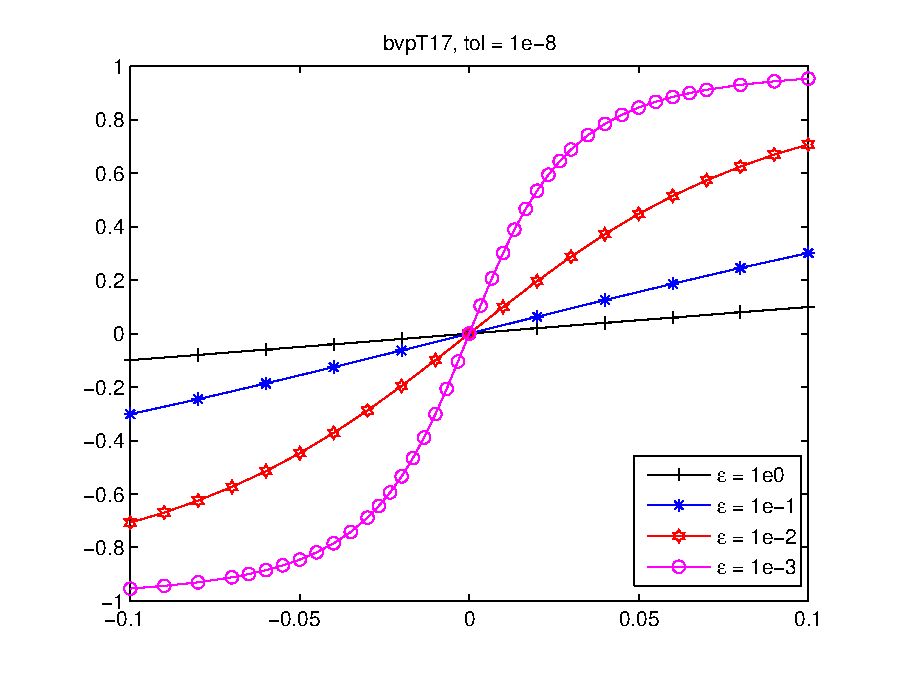
\includegraphics[height=6cm]{Prob17}}
\caption{Behavior of the solution of problem \ref{test17}.}
\end{figure}
\newpage
\subsection{Problem bvpT18}\label{test18}
The problem is 
\begin{eqnarray*}
\lambda z'' =  - z', \;\;\;z(0) = 1, \;\;\; z(1) = \exp(-1 /\lambda)
\end{eqnarray*}
with
\[
z \in \RR, \;\;\; t\in [0,1].
\]
We write this problem in first order form by defining $y_1=z$ and $y_2=z'$, yielding a system of differential equations of the form
\begin{equation*}
\left(\begin{array}{c}
y_1\\
y_2
\end{array}\right)'=
\left(\begin{array}{c}
y_2\\
\frac{1}{\lambda}f(y_2)
\end{array}\right),
\end{equation*}
where
\begin{equation*}
 f(z') = - z,
\end{equation*}
with
\[
(y_1,y_2)^T \in \RR^{2}, \;\;\;  t \in [0,1].
\]
The  boundary conditions are obtained from
\begin{equation*}
\left(
  \begin{array}{cc}
    1 & 0 \\
    0 & 0 \\
  \end{array}
\right)
\left(\begin{array}{c}
y_{1}(0)\\
y_{2}(0)
\end{array}\right)
+
\left(
  \begin{array}{cc}
    0 & 0 \\
    1 & 0 \\
  \end{array}
\right)
\left(\begin{array}{c}
y_{1}(1)\\
y_{2}(1)
\end{array}\right)=\left(\begin{array}{c}
1\\
\exp(-1 /\lambda)
\end{array}\right).
\end{equation*}
\textrm{Exact solution}
$$z(t) =   \exp(-t /\lambda).$$
The solution has a boundary layer of width $O(\lambda)$  at $t = 0.$

\begin{figure}[htb]
\centerline{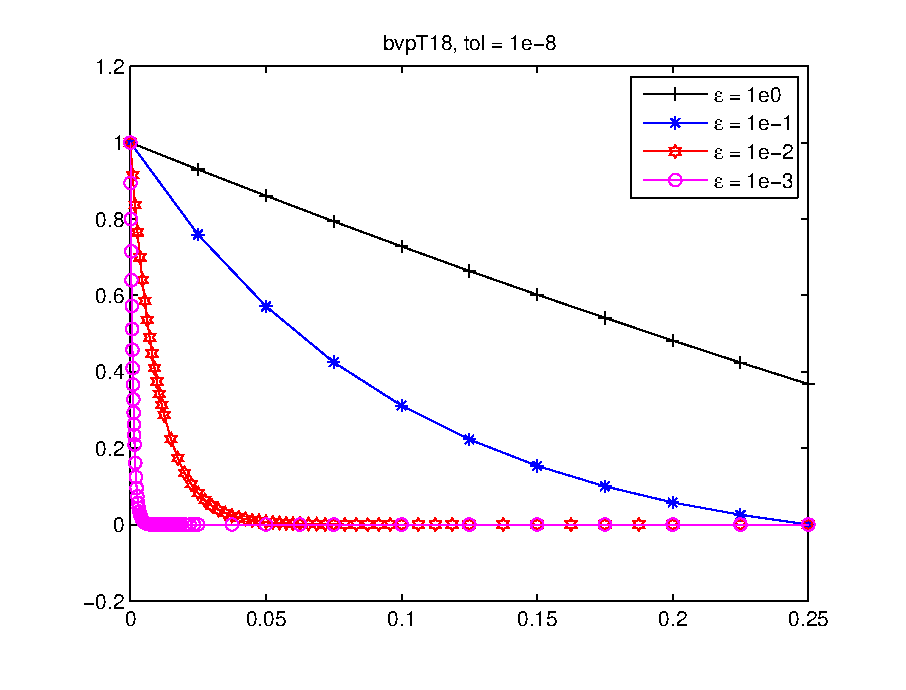
\includegraphics[height=6cm]{Prob18}}
\caption{Behavior of the solution of problem \ref{test18}.}
\end{figure}
\newpage
\section{Nonlinear Problems}\label{Nonlinear}
\subsection{Problem bvpT19}\label{test19}
The problem is
\begin{eqnarray*}
\lambda z'' =  -\exp(z) z' + \frac{\displaystyle{\pi}}{\displaystyle{2}} \sin(\pi t / 2) \exp(2z), \;\;\;z(0) = 0, \;\;\; z(1) =0
\end{eqnarray*}
with
\[
z \in \RR, \;\;\; t\in [0,1].
\]
We write this problem in first order form by defining $y_1=z$ and $y_2=z'$, yielding a system of differential equations of the form
\begin{equation*}
\left(\begin{array}{c}
y_1\\
y_2
\end{array}\right)'=
\left(\begin{array}{c}
y_2\\
\frac{1}{\lambda}f(t,y_1,y_2)
\end{array}\right),
\end{equation*}
where
\begin{equation*}
f(t,z,z') = -\exp(z) z' + \frac{\displaystyle{\pi}}{\displaystyle{2}} \sin(\pi t / 2) \exp(2z),
\end{equation*}
with
\[
(y_1,y_2)^T \in \RR^{2}, \;\;\;  t \in [0,1].
\]
The  boundary conditions are obtained from
\begin{equation*}
\left(
  \begin{array}{cc}
    1 & 0 \\
    0 & 0 \\
  \end{array}
\right)
\left(\begin{array}{c}
y_{1}(0)\\
y_{2}(0)
\end{array}\right)
+
\left(
  \begin{array}{cc}
    0 & 0 \\
    1 & 0 \\
  \end{array}
\right)
\left(\begin{array}{c}
y_{1}(1)\\
y_{2}(1)
\end{array}\right)=\left(\begin{array}{c}
0\\
0
\end{array}\right).
\end{equation*}

\begin{figure}[htb]
\centerline{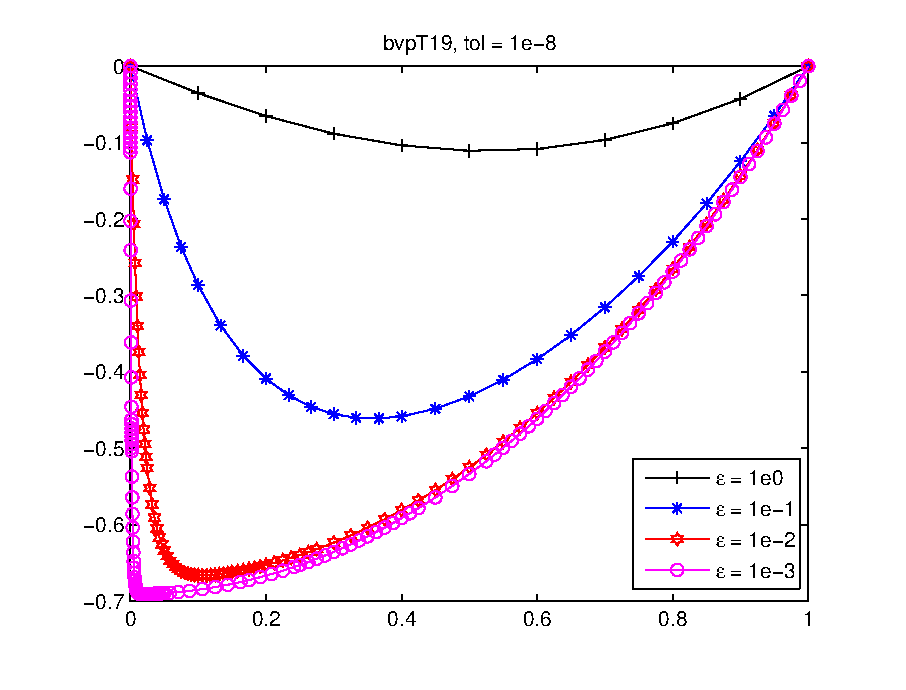
\includegraphics[height=6cm]{Prob19}}
\caption{Behavior of the solution of problem \ref{test19}.}
\end{figure}
\newpage
\subsection{Problem bvpT20}\label{test20}
The problem is 
\begin{eqnarray*}
\lambda z'' =  -(z')^{2} + 1, \;\;\;z(0) = 1 +\lambda \ln \cosh(-0.745 /\lambda), \;\;\; z(1) =1 +\lambda \ln \cosh(0.255 /\lambda)
\end{eqnarray*}
with
\[
z \in \RR, \;\;\; t\in [0,1].
\]
We write this problem in first order form by defining $y_1=z$ and $y_2=z'$, yielding a system of differential equations of the form
\begin{equation*}
\left(\begin{array}{c}
y_1\\
y_2
\end{array}\right)'=
\left(\begin{array}{c}
y_2\\
\frac{1}{\lambda}f(y_2)
\end{array}\right),
\end{equation*}
where
\begin{equation*}
 f(z') = -(z')^{2} + 1,
\end{equation*}
with
\[
(y_1,y_2)^T \in \RR^{2}, \;\;\;  t \in [0,1].
\]
The  boundary conditions are obtained from
\begin{equation*}
\left(
  \begin{array}{cc}
    1 & 0 \\
    0 & 0 \\
  \end{array}
\right)
\left(\begin{array}{c}
y_{1}(0)\\
y_{2}(0)
\end{array}\right)
+
\left(
  \begin{array}{cc}
    0 & 0 \\
    1 & 0 \\
  \end{array}
\right)
\left(\begin{array}{c}
y_{1}(1)\\
y_{2}(1)
\end{array}\right)=\left(\begin{array}{c}
1 +\lambda \ln \cosh(-0.745 /\lambda) \\
1 +\lambda \ln \cosh(0.255 /\lambda)
\end{array}\right).
\end{equation*}
\textrm{Exact solution}
$$z(t) = 1 +\lambda \ln \cosh(t - 0.745) /\lambda).$$
The solution has a corner layer at $t = 0.745.$

\begin{figure}[htb]
\centerline{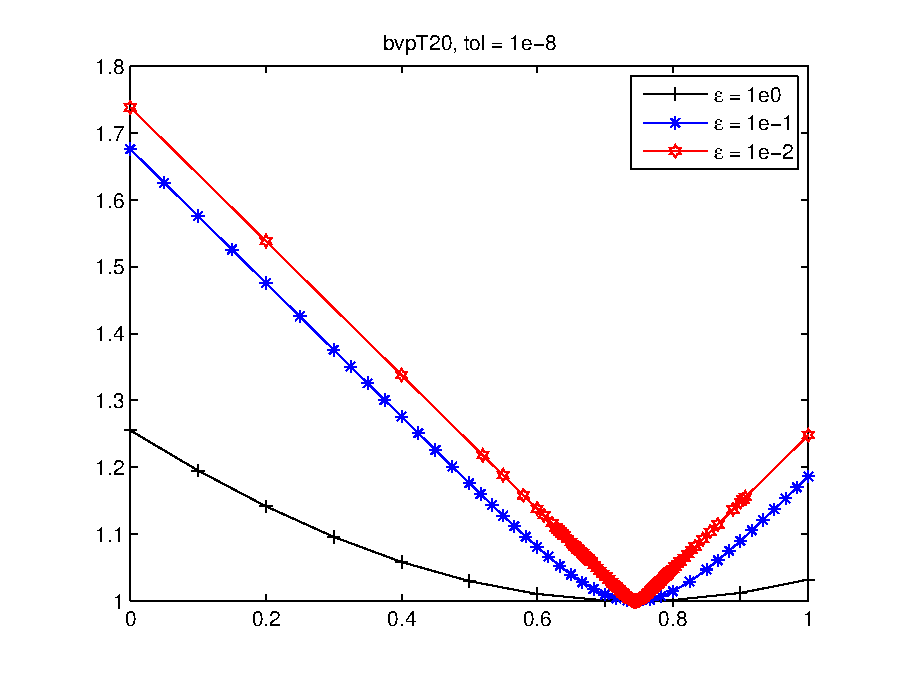
\includegraphics[height=6cm]{Prob20}}
\caption{Behavior of the solution of problem \ref{test20}.}
\end{figure}
\newpage
\subsection{Problem bvpT21}\label{test21}
The problem is 
\begin{eqnarray*}
\lambda z'' =   z +  z^{2} - \exp(-2 t / \sqrt{\lambda}), \;\;\;z(0) = 1, \;\;\; z(1) = \exp(-1 / \sqrt{\lambda})
\end{eqnarray*}
with
\[
z \in \RR, \;\;\; t\in [0,1].
\]
We write this problem in first order form by defining $y_1=z$ and $y_2=z'$, yielding a system of differential equations of the form
\begin{equation*}
\left(\begin{array}{c}
y_1\\
y_2
\end{array}\right)'=
\left(\begin{array}{c}
y_2\\
\frac{1}{\lambda}f(t,y_1)
\end{array}\right),
\end{equation*}
where
\begin{equation*}
f(t,z) = z +  z^{2} - \exp(-2 t / \sqrt{\lambda}),
\end{equation*}
with
\[
(y_1,y_2)^T \in \RR^{2}, \;\;\;  t \in [0,1].
\]
The  boundary conditions are obtained from
\begin{equation*}
\left(
  \begin{array}{cc}
    1 & 0 \\
    0 & 0 \\
  \end{array}
\right)
\left(\begin{array}{c}
y_{1}(0)\\
y_{2}(0)
\end{array}\right)
+
\left(
  \begin{array}{cc}
    0 & 0 \\
    1 & 0 \\
  \end{array}
\right)
\left(\begin{array}{c}
y_{1}(1)\\
y_{2}(1)
\end{array}\right)=\left(\begin{array}{c}
1  \\
\exp(-1 / \sqrt{\lambda})
\end{array}\right).
\end{equation*}
\textrm{Exact solution}
$$z(t) =  \exp(-t / \sqrt{\lambda}).$$
The solution has a boundary layer of width $O(\sqrt\lambda)$  at $t = 0.$

\begin{figure}[htb]
\centerline{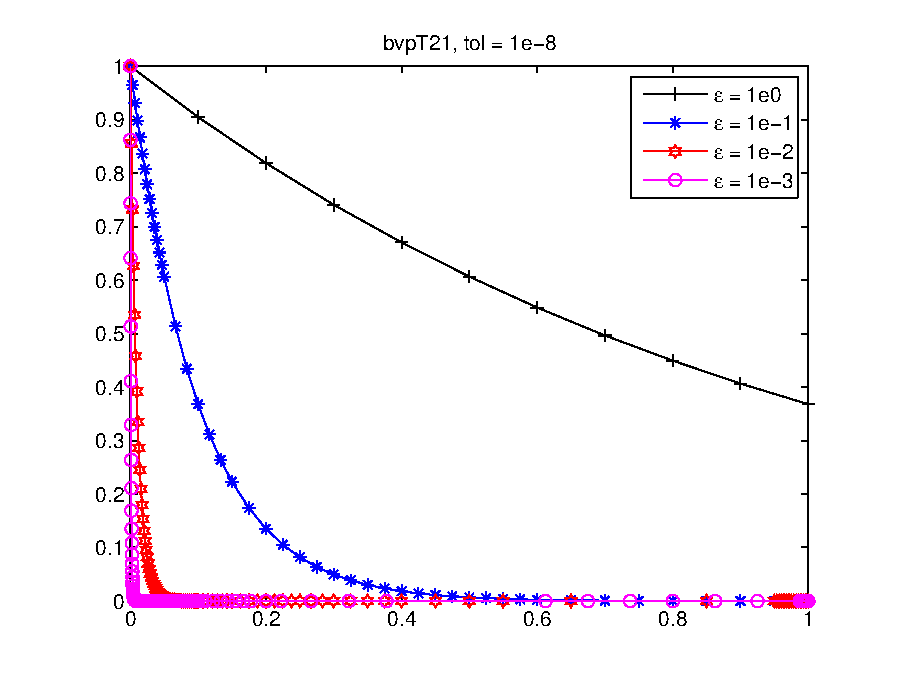
\includegraphics[height=6cm]{Prob21}}
\caption{Behavior of the solution of problem \ref{test21}.}
\end{figure}
 \newpage
\subsection{Problem bvpT22}\label{test22}
The problem is 
\begin{eqnarray*}
\lambda z'' = - z' -  z^{2}, \;\;\;z(0) = 0, \;\;\; z(1) = \frac{1}{2}
\end{eqnarray*}
with
\[
z \in \RR, \;\;\; t\in [0,1].
\]
We write this problem in first order form by defining $y_1=z$ and $y_2=z'$, yielding a system of differential equations of the form
\begin{equation*}
\left(\begin{array}{c}
y_1\\
y_2
\end{array}\right)'=
\left(\begin{array}{c}
y_2\\
\frac{1}{\lambda}f(y_1,y_2)
\end{array}\right),
\end{equation*}
where
\begin{equation*}
f(z,z') = - z' -  z^{2},
\end{equation*}
with
\[
(y_1,y_2)^T \in \RR^{2}, \;\;\;  t \in [0,1].
\]
The  boundary conditions are obtained from
\begin{equation*}
\left(
  \begin{array}{cc}
    1 & 0 \\
    0 & 0 \\
  \end{array}
\right)
\left(\begin{array}{c}
y_{1}(0)\\
y_{2}(0)
\end{array}\right)
+
\left(
  \begin{array}{cc}
    0 & 0 \\
    1 & 0 \\
  \end{array}
\right)
\left(\begin{array}{c}
y_{1}(1)\\
y_{2}(1)
\end{array}\right)=\left(\begin{array}{c}
0 \\
\frac{1}{2}
\end{array}\right).
\end{equation*}
The solution has a boundary layer near $t = 0.$

\begin{figure}[htb]
\centerline{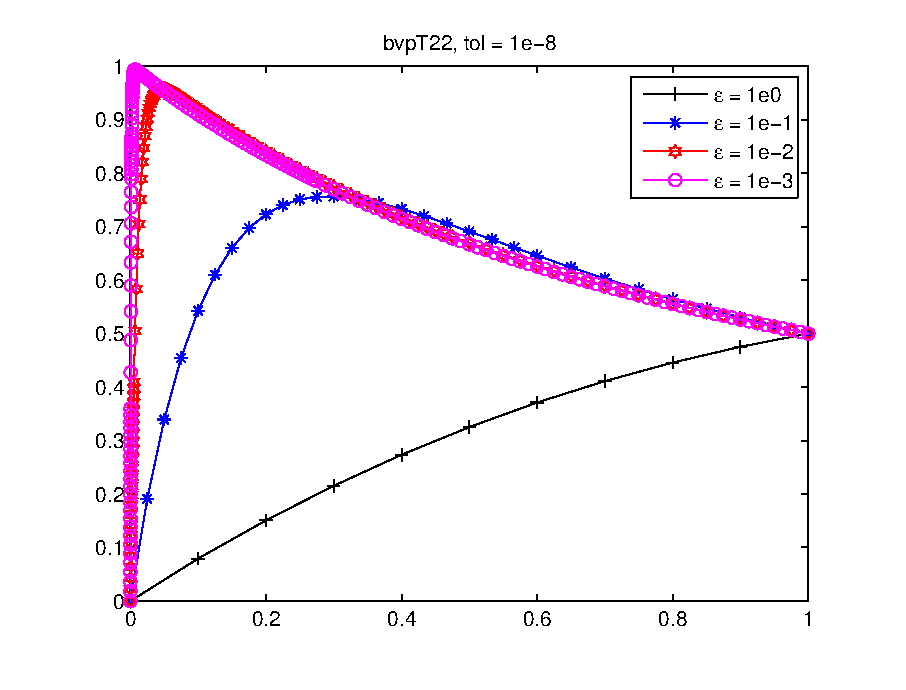
\includegraphics[height=6cm]{Prob22}}
\caption{Behavior of the solution of problem \ref{test22}.}
\end{figure}
\newpage
\subsection{Problem bvpT23}\label{test23}
The problem is 
\begin{eqnarray*}
z'' = \lambda \sinh(\lambda z), \;\;\;z(0) = 0, \;\;\; z(1) = 1
\end{eqnarray*}
with
\[
z \in \RR, \;\;\; t\in [0,1].
\]
We write this problem in first order form by defining $y_1=z$ and $y_2=z'$, yielding a system of differential equations of the form
\begin{equation*}
\left(\begin{array}{c}
y_1\\
y_2
\end{array}\right)'=
\left(\begin{array}{c}
y_2\\
f(y_1)
\end{array}\right),
\end{equation*}
where
\begin{equation*}
f(z) =\lambda \sinh(\lambda z),
\end{equation*}
with
\[
(y_1,y_2)^T \in \RR^{2}, \;\;\;  t \in [0,1].
\]
The  boundary conditions are obtained from
\begin{equation*}
\left(
  \begin{array}{cc}
    1 & 0 \\
    0 & 0 \\
  \end{array}
\right)
\left(\begin{array}{c}
y_{1}(0)\\
y_{2}(0)
\end{array}\right)
+
\left(
  \begin{array}{cc}
    0 & 0 \\
    1 & 0 \\
  \end{array}
\right)
\left(\begin{array}{c}
y_{1}(1)\\
y_{2}(1)
\end{array}\right)=\left(\begin{array}{c}
0 \\
1
\end{array}\right).
\end{equation*}
The solution has a boundary layer near $t = 1.$

\begin{figure}[htb]
\centerline{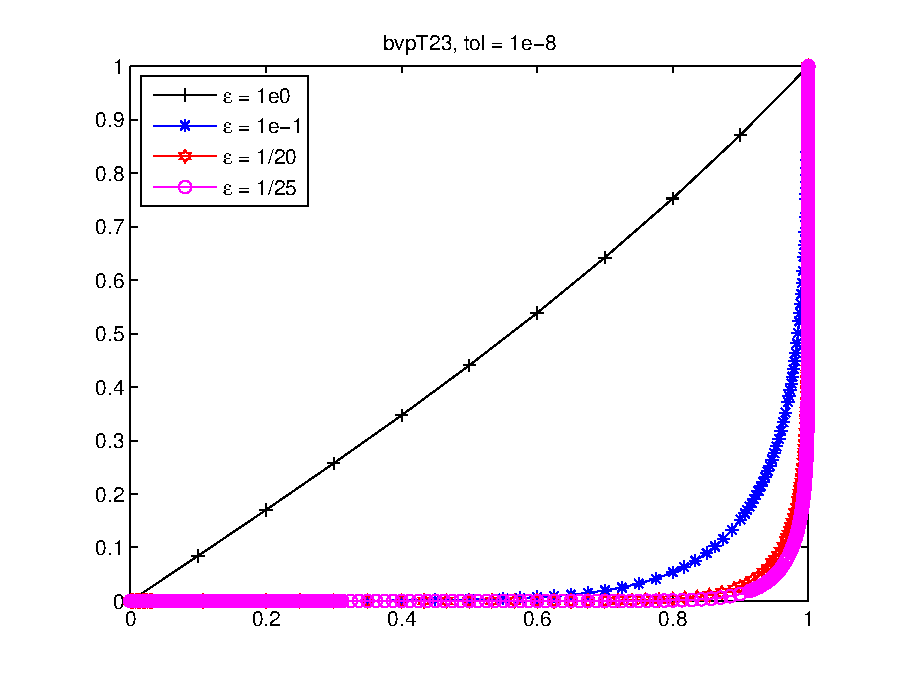
\includegraphics[height=6cm]{Prob23}}
\caption{Behavior of the solution of problem \ref{test23}.}
\end{figure}
\newpage
\subsection{Problem bvpT24}\label{test24}
The problem is 
\begin{equation*}
\begin{array}{ll}
\lambda A(t) z z''  = \Big(\frac{\displaystyle{1 + \gamma}}{\displaystyle{2}} -\lambda A'(t)\Big) z z^{'} - \frac{\displaystyle{z'}}{\displaystyle{z}}
- \frac{\displaystyle{A'(t)}}{\displaystyle{A(t)}} \Big(1 - \big(\frac{\displaystyle{\gamma - 1}}{\displaystyle{2}}\big) z^2 \Big) ,  &\\
A(t) = 1 + t^{2}, \;\;\;  \gamma = 1.4, \;\;\;z(0) =0.9129, \;\;\; z(1) = 0.375 \\
   \end{array}
\end{equation*}
with
\[
z \in \RR, \;\;\; t\in [0,1].
\]
We write this problem in first order form by defining $y_1=z$ and $y_2=z'$, yielding a system of differential equations of the form
\begin{equation*}
\left(\begin{array}{c}
y_1\\
y_2
\end{array}\right)'=
\left(\begin{array}{c}
y_2\\
\frac{1}{\lambda A(t) y_1}f(t,y_1,y_2)
\end{array}\right),
\end{equation*}
where
\begin{equation*}
f(t,z,z') = \Big(\frac{\displaystyle{1 + \gamma}}{\displaystyle{2}} -\lambda A'(t)\Big) z z^{'} - \frac{\displaystyle{z'}}{\displaystyle{z}}
- \frac{\displaystyle{A'(t)}}{\displaystyle{A(t)}} \Big(1 - \big(\frac{\displaystyle{\gamma - 1}}{\displaystyle{2}}\big) z^2 \Big),
\end{equation*}
with
\[
(y_1,y_2)^T \in \RR^{2}, \;\;\;  t \in [0,1].
\]
The  boundary conditions are obtained from
\begin{equation*}
\left(
  \begin{array}{cc}
    1 & 0 \\
    0 & 0 \\
  \end{array}
\right)
\left(\begin{array}{c}
y_{1}(0)\\
y_{2}(0)
\end{array}\right)
+
\left(
  \begin{array}{cc}
    0 & 0 \\
    1 & 0 \\
  \end{array}
\right)
\left(\begin{array}{c}
y_{1}(1)\\
y_{2}(1)
\end{array}\right)=\left(\begin{array}{c}
0.9129 \\
0.375
\end{array}\right).
\end{equation*}
This equation represents a shock wave in a one dimensional nozzle flow.

\begin{figure}[htb]
\centerline{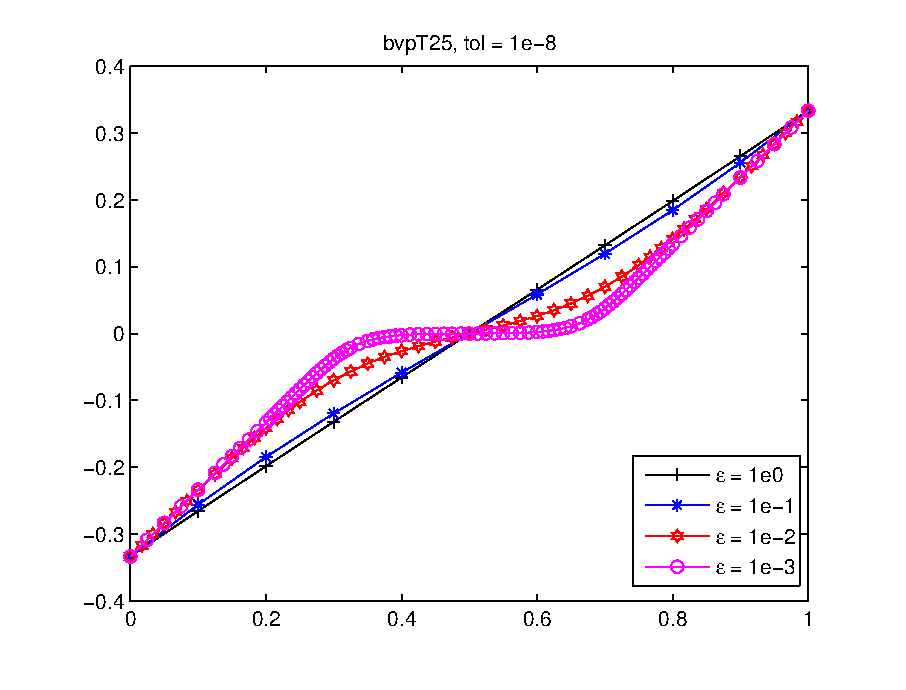
\includegraphics[height=6cm]{Prob25}}
\caption{Behavior of the solution of problem \ref{test24}.}
\end{figure}
\newpage
\subsection{Problem bvpT25}\label{test25}
The problem is 
\begin{eqnarray*}
\lambda z'' = - z z' +  z , \;\;\;z(0) = -\frac{1}{3}, \;\;\; z(1) = \frac{1}{3}
\end{eqnarray*}
with
\[
z \in \RR, \;\;\; t\in [0,1].
\]
We write this problem in first order form by defining $y_1=z$ and $y_2=z'$, yielding a system of differential equations of the form
\begin{equation*}
\left(\begin{array}{c}
y_1\\
y_2
\end{array}\right)'=
\left(\begin{array}{c}
y_2\\
\frac{1}{\lambda}f(y_1,y_2)
\end{array}\right),
\end{equation*}
where
\begin{equation*}
f(z,z') = - z z' +  z,
\end{equation*}
with
\[
(y_1,y_2)^T \in \RR^{2}, \;\;\;  t \in [0,1].
\]
The  boundary conditions are obtained from
\begin{equation*}
\left(
  \begin{array}{cc}
    1 & 0 \\
    0 & 0 \\
  \end{array}
\right)
\left(\begin{array}{c}
y_{1}(0)\\
y_{2}(0)
\end{array}\right)
+
\left(
  \begin{array}{cc}
    0 & 0 \\
    1 & 0 \\
  \end{array}
\right)
\left(\begin{array}{c}
y_{1}(1)\\
y_{2}(1)
\end{array}\right)=\left(\begin{array}{c}
-\frac{1}{3} \\
\frac{1}{3}
\end{array}\right).
\end{equation*}
The solution has corner layers at $t= \frac{1}{3}$ and $t= \frac{2}{3}.$

\begin{figure}[htb]
\centerline{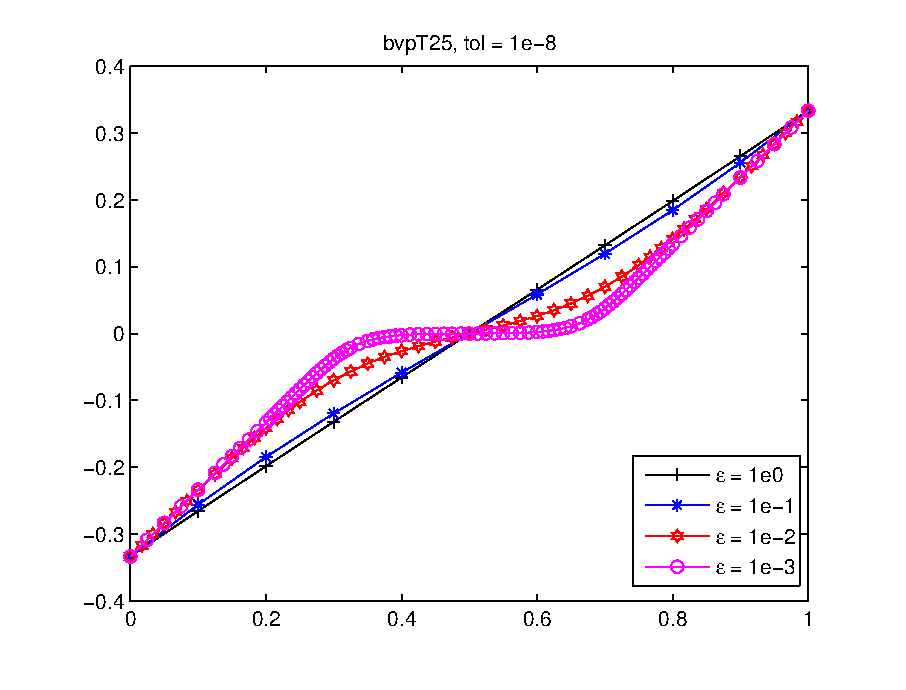
\includegraphics[height=6cm]{Prob25}}
\caption{Behavior of the solution of problem \ref{test25}.}
\end{figure}
\newpage
\subsection{Problem bvpT26}\label{test26}
The problem is 
\begin{eqnarray*}
\lambda z'' = - z z' +  z , \;\;\;z(0) =1, \;\;\; z(1) = -\frac{1}{3}
\end{eqnarray*}
with
\[
z \in \RR, \;\;\; t\in [0,1].
\]
We write this problem in first order form by defining $y_1=z$ and $y_2=z'$, yielding a system of differential equations of the form
\begin{equation*}
\left(\begin{array}{c}
y_1\\
y_2
\end{array}\right)'=
\left(\begin{array}{c}
y_2\\
\frac{1}{\lambda}f(y_1,y_2)
\end{array}\right),
\end{equation*}
where
\begin{equation*}
f(z,z') = - z z' +  z,
\end{equation*}
with
\[
(y_1,y_2)^T \in \RR^{2}, \;\;\;  t \in [0,1].
\]
The  boundary conditions are obtained from
\begin{equation*}
\left(
  \begin{array}{cc}
    1 & 0 \\
    0 & 0 \\
  \end{array}
\right)
\left(\begin{array}{c}
y_{1}(0)\\
y_{2}(0)
\end{array}\right)
+
\left(
  \begin{array}{cc}
    0 & 0 \\
    1 & 0 \\
  \end{array}
\right)
\left(\begin{array}{c}
y_{1}(1)\\
y_{2}(1)
\end{array}\right)=\left(\begin{array}{c}
1 \\
-\frac{1}{3}
\end{array}\right).
\end{equation*}
The solution has corner layers at $t= 0$ and $t= 1.$

\begin{figure}[htb]
\centerline{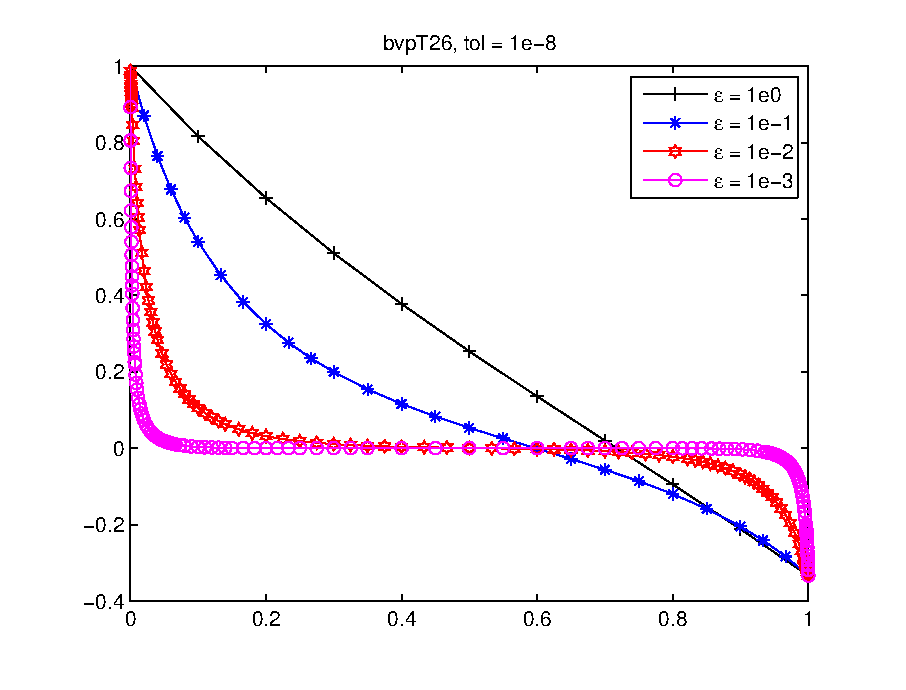
\includegraphics[height=6cm]{Prob26}}
\caption{Behavior of the solution of problem \ref{test26}.}
\end{figure}
\newpage
\subsection{Problem bvpT27}\label{test27}
The problem is 
\begin{eqnarray*}
\lambda z'' = - z z' +  z , \;\;\;z(0) =1, \;\;\; z(1) = \frac{1}{3}
\end{eqnarray*}
with
\[
z \in \RR, \;\;\; t\in [0,1].
\]
We write this problem in first order form by defining $y_1=z$ and $y_2=z'$, yielding a system of differential equations of the form
\begin{equation*}
\left(\begin{array}{c}
y_1\\
y_2
\end{array}\right)'=
\left(\begin{array}{c}
y_2\\
\frac{1}{\lambda}f(y_1,y_2)
\end{array}\right),
\end{equation*}
where
\begin{equation*}
f(z,z') = - z z' +  z,
\end{equation*}
with
\[
(y_1,y_2)^T \in \RR^{2}, \;\;\;  t \in [0,1].
\]
The  boundary conditions are obtained from
\begin{equation*}
\left(
  \begin{array}{cc}
    1 & 0 \\
    0 & 0 \\
  \end{array}
\right)
\left(\begin{array}{c}
y_{1}(0)\\
y_{2}(0)
\end{array}\right)
+
\left(
  \begin{array}{cc}
    0 & 0 \\
    1 & 0 \\
  \end{array}
\right)
\left(\begin{array}{c}
y_{1}(1)\\
y_{2}(1)
\end{array}\right)=\left(\begin{array}{c}
1 \\
\frac{1}{3}
\end{array}\right).
\end{equation*}
The solution has corner layers at $t= 0$ and a corner layer at $t= \frac{2}{3}.$

\begin{figure}[htb]
\centerline{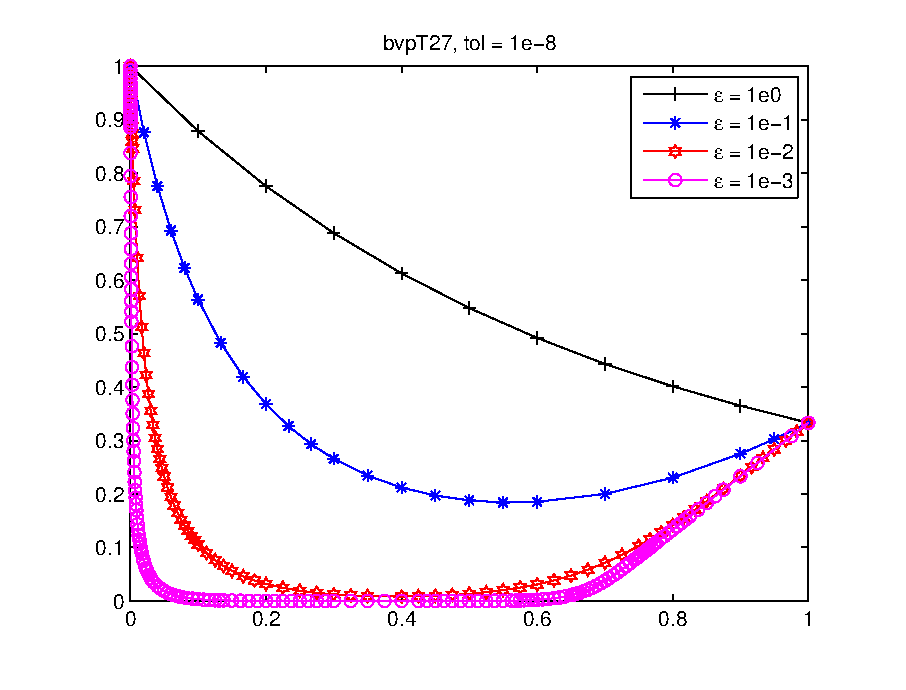
\includegraphics[height=6cm]{Prob27}}
\caption{Behavior of the solution of problem \ref{test27}.}
\end{figure}
\newpage
\subsection{Problem bvpT28}\label{test28}
The problem is 
\begin{eqnarray*}
\lambda z'' = - z z' +  z , \;\;\;z(0) =1, \;\;\; z(1) = \frac{3}{2}
\end{eqnarray*}
with
\[
z \in \RR, \;\;\; t\in [0,1].
\]
We write this problem in first order form by defining $y_1=z$ and $y_2=z'$, yielding a system of differential equations of the form
\begin{equation*}
\left(\begin{array}{c}
y_1\\
y_2
\end{array}\right)'=
\left(\begin{array}{c}
y_2\\
\frac{1}{\lambda}f(y_1,y_2)
\end{array}\right),
\end{equation*}
where
\begin{equation*}
 f(z,z') = - z z' +  z,
\end{equation*}
with
\[
(y_1,y_2)^T \in \RR^{2}, \;\;\;  t \in [0,1].
\]
The  boundary conditions are obtained from
\begin{equation*}
\left(
  \begin{array}{cc}
    1 & 0 \\
    0 & 0 \\
  \end{array}
\right)
\left(\begin{array}{c}
y_{1}(0)\\
y_{2}(0)
\end{array}\right)
+
\left(
  \begin{array}{cc}
    0 & 0 \\
    1 & 0 \\
  \end{array}
\right)
\left(\begin{array}{c}
y_{1}(1)\\
y_{2}(1)
\end{array}\right)=\left(\begin{array}{c}
1 \\
\frac{3}{2}
\end{array}\right).
\end{equation*}
The solution has corner layers at $t= 0.$

\begin{figure}[htb]
\centerline{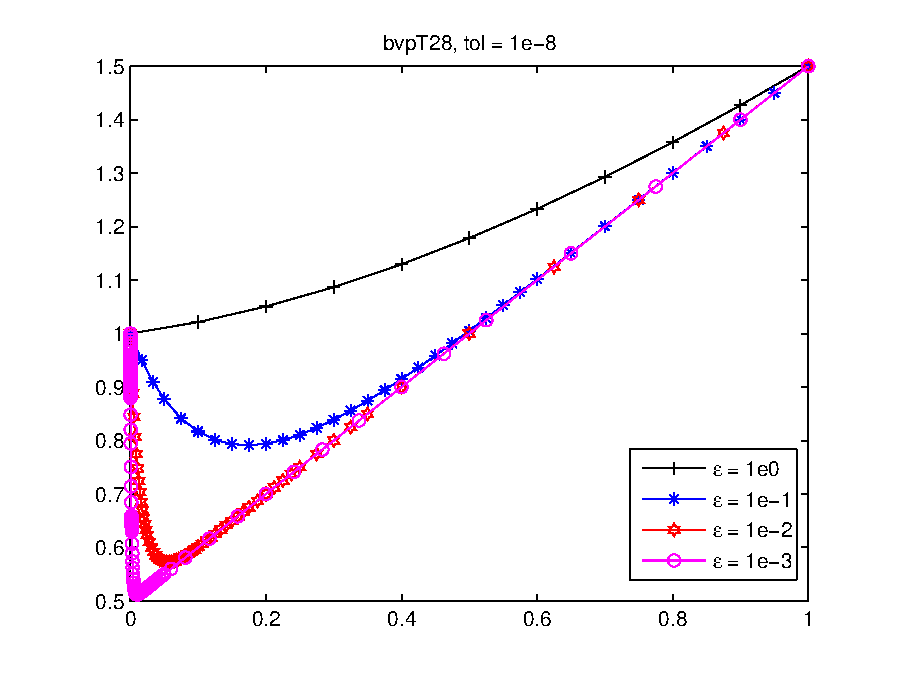
\includegraphics[height=6cm]{Prob28}}
\caption{Behavior of the solution of problem \ref{test28}.}
\end{figure}
\newpage
\subsection{Problem bvpT29}\label{test29}
The problem is 
\begin{eqnarray*}
\lambda z'' = - z z' +  z , \;\;\;z(0) =0, \;\;\; z(1) = \frac{3}{2}
\end{eqnarray*}
with
\[
z \in \RR, \;\;\; t\in [0,1].
\]
We write this problem in first order form by defining $y_1=z$ and $y_2=z'$, yielding a system of differential equations of the form
\begin{equation*}
\left(\begin{array}{c}
y_1\\
y_2
\end{array}\right)'=
\left(\begin{array}{c}
y_2\\
\frac{1}{\lambda}f(y_1,y_2)
\end{array}\right),
\end{equation*}
where
\begin{equation*}
 f(z,z') = - z z' +  z,
\end{equation*}
with
\[
(y_1,y_2)^T \in \RR^{2}, \;\;\;  t \in [0,1].
\]
The  boundary conditions are obtained from
\begin{equation*}
\left(
  \begin{array}{cc}
    1 & 0 \\
    0 & 0 \\
  \end{array}
\right)
\left(\begin{array}{c}
y_{1}(0)\\
y_{2}(0)
\end{array}\right)
+
\left(
  \begin{array}{cc}
    0 & 0 \\
    1 & 0 \\
  \end{array}
\right)
\left(\begin{array}{c}
y_{1}(1)\\
y_{2}(1)
\end{array}\right)=\left(\begin{array}{c}
0 \\
\frac{3}{2}
\end{array}\right).
\end{equation*}
The solution has corner layers at $t= 0.$

\begin{figure}[htb]
\centerline{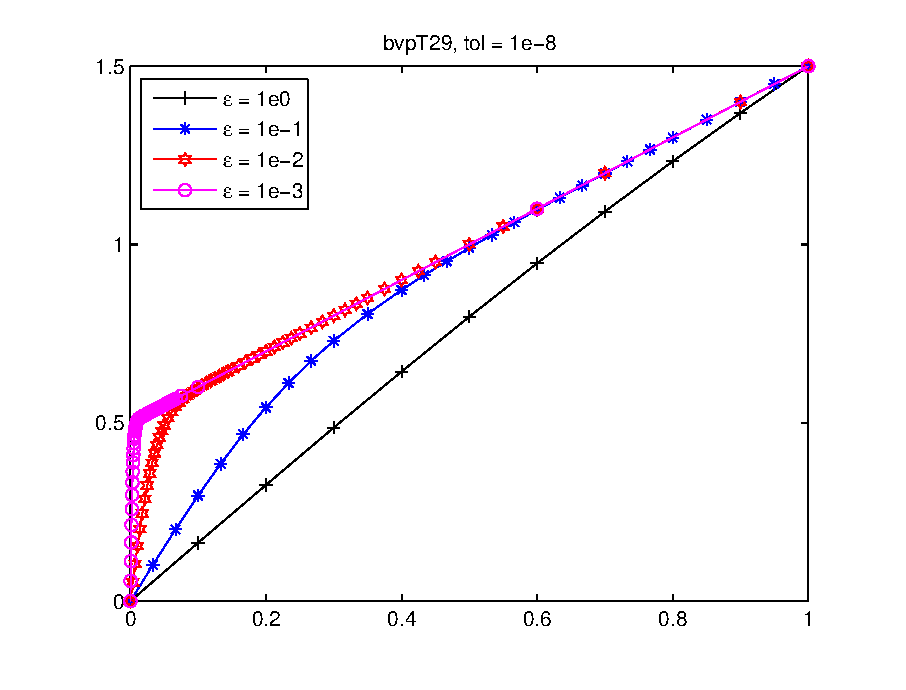
\includegraphics[height=6cm]{Prob29}}
\caption{Behavior of the solution of problem \ref{test29}.}
\end{figure}
\newpage
\subsection{Problem bvpT30}\label{test30}
The problem is
\begin{eqnarray*}
\lambda z'' = - z z' +  z , \;\;\;z(0) =-\frac{7}{6}, \;\;\; z(1) = \frac{3}{2}
\end{eqnarray*}
with
\[
z \in \RR, \;\;\; t\in [0,1].
\]
We write this problem in first order form by defining $y_1=z$ and $y_2=z'$, yielding a system of differential equations of the form
\begin{equation*}
\left(\begin{array}{c}
y_1\\
y_2
\end{array}\right)'=
\left(\begin{array}{c}
y_2\\
\frac{1}{\lambda}f(y_1,y_2)
\end{array}\right),
\end{equation*}
where
\begin{equation*}
f(z,z') = - z z' +  z,
\end{equation*}
with
\[
(y_1,y_2)^T \in \RR^{2}, \;\;\;  t \in [0,1].
\]
The  boundary conditions are obtained from
\begin{equation*}
\left(
  \begin{array}{cc}
    1 & 0 \\
    0 & 0 \\
  \end{array}
\right)
\left(\begin{array}{c}
y_{1}(0)\\
y_{2}(0)
\end{array}\right)
+
\left(
  \begin{array}{cc}
    0 & 0 \\
    1 & 0 \\
  \end{array}
\right)
\left(\begin{array}{c}
y_{1}(1)\\
y_{2}(1)
\end{array}\right)=\left(\begin{array}{c}
-\frac{7}{6} \\
\frac{3}{2}
\end{array}\right).
\end{equation*}
The solution has a shock layer  at $t= \frac{1}{3}.$

\begin{figure}[htb]
\centerline{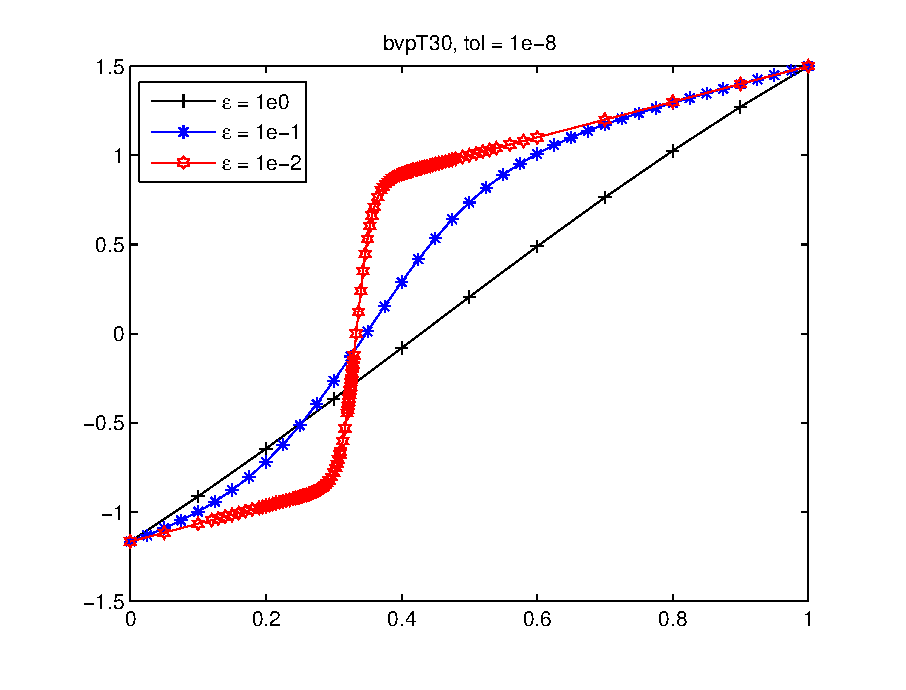
\includegraphics[height=6cm]{Prob30}}
\caption{Behavior of the solution of problem \ref{test30}.}
\end{figure}
\newpage
\subsection{Problem bvpT31}\label{test31}
The problem is 
\begin{eqnarray*}
\begin{array}{ll}
z' = \sin \theta,\, \theta' = M,\, \lambda M' = -Q,\, \lambda Q' = (z-1) \cos \theta - MT,\, T = \sec \theta + \lambda Q \tan \theta,  &\\
z(0) = z(1) = 0, \, M(0) = M(1) = 0. \\
\end{array}
\end{eqnarray*}
with
\[
z \in \RR, \;\;\; t\in [0,1].
\]
We write this problem in first order form by defining $y_1=z,\,y_2 = \theta,\,y_3 = M$ and $y_4 = Q$, yielding a system of differential equations of the form
\begin{equation*}
\left(\begin{array}{c}
y_1\\
y_2\\
y_3\\
y_4
\end{array}\right)'=
\left(\begin{array}{c}
\sin y_2 \\
y_3\\
- y_4/ \lambda\\
f(y_1,y_2,y_3,y_4)
\end{array}\right),
\end{equation*}
where
\begin{equation*}
f(z,\theta,M,Q ) = \frac{1}{\lambda}((z - 1) \cos \theta - M \sec \theta) + \lambda Q \tan \theta)
\end{equation*}
with
\[
(y_1,y_2,y_3,y_4)^T \in \RR^{4}, \;\;\;  t \in [0,1].
\]
The  boundary conditions are obtained from
\begin{equation*}
\left(
  \begin{array}{cccc}
    1& 0 & 0 & 0\\
    0 & 0 & 1 & 0\\
    0 & 0 & 0 & 0\\
    0 & 0 & 0 & 0\\
  \end{array}
\right)
\left(\begin{array}{c}
y_{1}(0)\\
y_{2}(0)\\
y_{3}(0)\\
y_{4}(0)
\end{array}\right)
+
\left(
  \begin{array}{cccc}
    0 & 0 & 0 & 0\\
    0 & 0 & 0 & 0\\
    1 & 0 & 0 & 0\\
    0 & 0 & 1 & 0\\
  \end{array}
\right)
\left(\begin{array}{c}
y_{1}(1)\\
y_{2}(1)\\
y_{3}(1)\\
y_{4}(1)
\end{array}\right)=\left(\begin{array}{c}
0 \\
0 \\
0\\
0
\end{array}\right).
\end{equation*}
This equation models nonlinear elastic beams.

\begin{figure}[htb]
\centerline{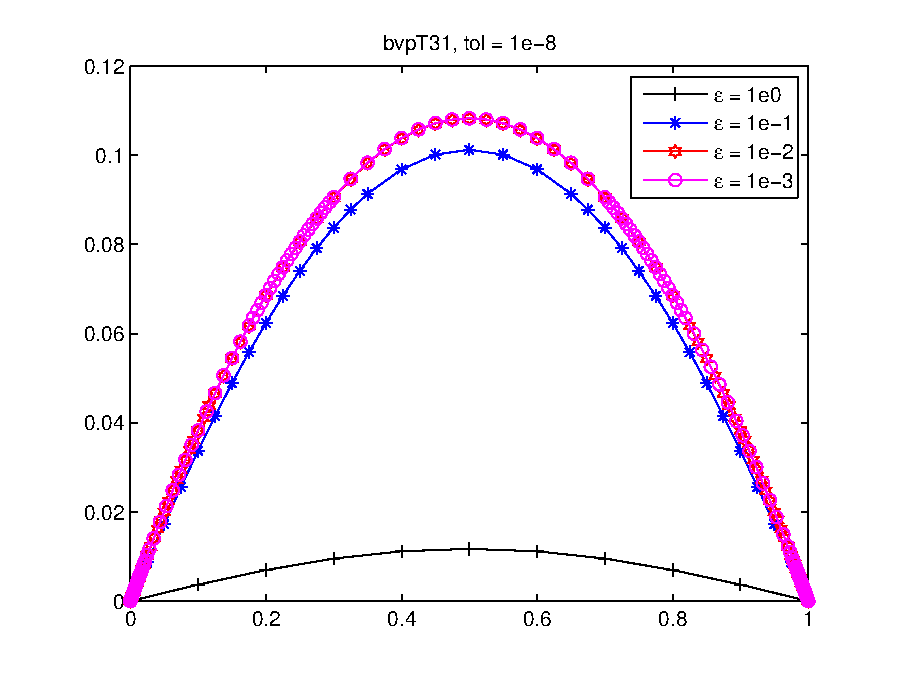
\includegraphics[height=6cm]{Prob31}}
\caption{Behavior of the solution of problem \ref{test31}.}
\end{figure}
\newpage
\subsection{Problem bvpT32}\label{test32}
The problem is 
\begin{eqnarray*}
z'''' =\lambda( z' z'' -  z z''') , \;\;\;z(0) =z'(0) = 0, \;\;\; z(1) = 1,\;\;\; z'(1) = 0
\end{eqnarray*}
with
\[
z \in \RR, \;\;\; t\in [0,1].
\]
We write this problem in first order form by defining $y_1=z,\,y_2 = z',\,y_3 = z''$ and $y_4 = z'''$, yielding a system of differential equations of the form
\begin{equation*}
\left(\begin{array}{c}
y_1\\
y_2\\
y_3\\
y_4
\end{array}\right)'=
\left(\begin{array}{c}
y_2\\
y_3\\
y_4\\
f(y_1,y_2,y_3,y_4)
\end{array}\right),
\end{equation*}
where
\begin{equation*}
f(z,z',z'',z''') = \lambda( z' z'' -  z z'''),
\end{equation*}
with
\[
(y_1,y_2,y_3,y_4)^T \in \RR^{4}, \;\;\;  t \in [0,1].
\]
The  boundary conditions are obtained from
\begin{equation*}
\left(
  \begin{array}{cccc}
    1 & 0 & 0 & 0\\
    0 & 1 & 0 & 0\\
    0 & 0 & 0 & 0\\
    0 & 0 & 0 & 0\\
  \end{array}
\right)
\left(\begin{array}{c}
y_{1}(0)\\
y_{2}(0)\\
y_{3}(0)\\
y_{4}(0)
\end{array}\right)
+
\left(
  \begin{array}{cccc}
    0 & 0 & 0 & 0\\
    0 & 0 & 0 & 0\\
    1 & 0 & 0 & 0\\
    0 & 1 & 0 & 0\\
  \end{array}
\right)
\left(\begin{array}{c}
y_{1}(1)\\
y_{2}(1)\\
y_{3}(1)\\
y_{4}(1)
\end{array}\right)=\left(\begin{array}{c}
0 \\
0 \\
1\\
0
\end{array}\right).
\end{equation*}
This problem arises from fluid injection through one side of a long vertical
channel

\begin{figure}[htb]
\centerline{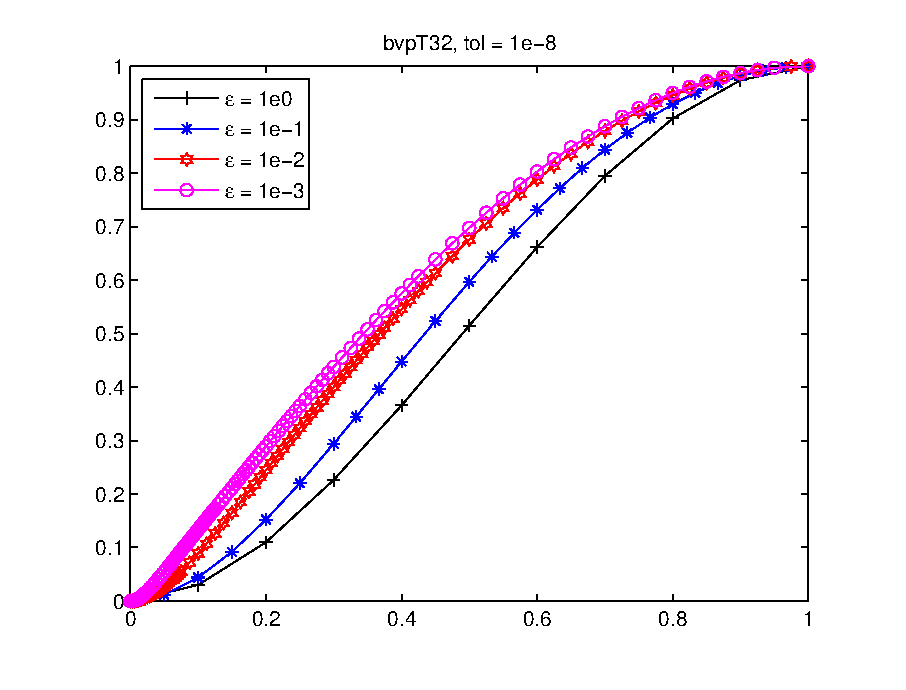
\includegraphics[height=6cm]{Prob32}}
\caption{Behavior of the solution of problem \ref{test32}.}
\end{figure}
\newpage
\subsection{Problem bvpT33}\label{test33}
The problem is 
\begin{eqnarray*}
\lambda z'''' =  -  z z''' - y y',\,\,  \lambda y'' = y z' - z y',\;\;\;y(0) =-1,\, y(1) = 1, \;\;\; z(0) =z'(0) = z(1) =z'(1) = 0,
\end{eqnarray*}
with
\[
z,y \in \RR, \;\;\; t\in [0,1].
\]
We write this problem in first order form by defining $y_1=y,\,y_2 = y',\,y_3 = z,\,y_4 = z',\, y_5 = z''$ and $y_6 = z''',$ yielding a system of differential equations of the form
\begin{equation*}
\left(\begin{array}{c}
y_1\\
y_2\\
y_3\\
y_4\\
y_5\\
y_6
\end{array}\right)'=
\left(\begin{array}{c}
y_2\\
\frac{1}{\lambda}y_1 y_4 - y_3 y_2\\
y_4\\
y_5\\
y_6\\
\frac{1}{\lambda}(-y_3 y_6 - y_1 y_2 )
\end{array}\right),
\end{equation*}
with
\[
(y_1,y_2,y_3,y_4,y_5,y_6)^T \in \RR^{6}, \;\;\;  t \in [0,1].
\]
The  boundary conditions are obtained from
\begin{equation*}
\left(
  \begin{array}{cccccc}
    1 & 0 & 0 & 0&0 & 0\\
    0 & 0 & 1 & 0&0 & 0\\
    0 & 0 & 0 & 1&0 & 0\\
    0 & 0 & 0 & 0&0 & 0\\
    0 & 0 & 0 & 0&0 & 0\\
    0 & 0 & 0 & 0&0 & 0 \end{array}
\right)
\left(\begin{array}{c}
y_{1}(0)\\
y_{2}(0)\\
y_{3}(0)\\
y_{4}(0)\\
y_{5}(0)\\
y_{6}(0)
\end{array}\right)
+
\left(
  \begin{array}{cccccc}
    0 & 0 & 0 & 0&0 & 0\\ 0 & 0 & 0 & 0&0 & 0\\ 0 & 0 & 0 & 0&0 & 0\\ 1 & 0 & 0 & 0&0 & 0\\ 0 & 0 & 1 & 0&0 & 0\\
    0 & 0 & 0 & 1&0 & 0 \end{array}
\right)
\left(\begin{array}{c}
y_{1}(1)\\
y_{2}(1)\\
y_{3}(1)\\
y_{4}(1) \\
y_{5}(1) \\
y_{6}(1)
\end{array}\right)=\left(\begin{array}{c}
-1 \\
0 \\
0\\
1\\
0\\
0
\end{array}\right).
\end{equation*}

\begin{figure}[htb]
\centerline{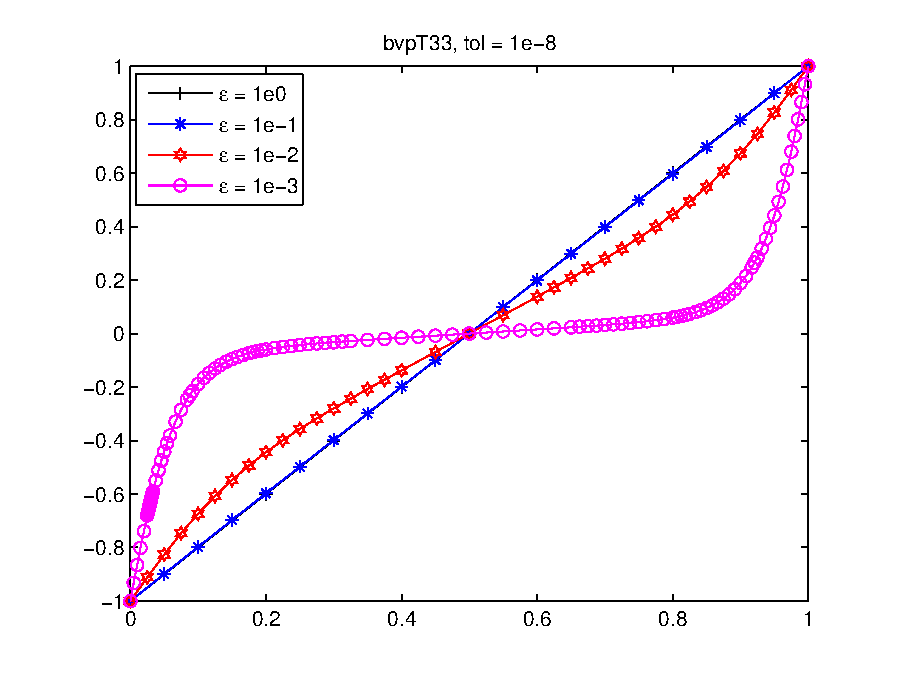
\includegraphics[height=6cm]{Prob33}}
\caption{Behavior of the solution of problem \ref{test33}.}
\end{figure}

\end{document} 